% Options for packages loaded elsewhere
\PassOptionsToPackage{unicode}{hyperref}
\PassOptionsToPackage{hyphens}{url}
%
\documentclass[
]{book}
\usepackage{lmodern}
\usepackage{amssymb,amsmath}
\usepackage{ifxetex,ifluatex}
\ifnum 0\ifxetex 1\fi\ifluatex 1\fi=0 % if pdftex
  \usepackage[T1]{fontenc}
  \usepackage[utf8]{inputenc}
  \usepackage{textcomp} % provide euro and other symbols
\else % if luatex or xetex
  \usepackage{unicode-math}
  \defaultfontfeatures{Scale=MatchLowercase}
  \defaultfontfeatures[\rmfamily]{Ligatures=TeX,Scale=1}
\fi
% Use upquote if available, for straight quotes in verbatim environments
\IfFileExists{upquote.sty}{\usepackage{upquote}}{}
\IfFileExists{microtype.sty}{% use microtype if available
  \usepackage[]{microtype}
  \UseMicrotypeSet[protrusion]{basicmath} % disable protrusion for tt fonts
}{}
\makeatletter
\@ifundefined{KOMAClassName}{% if non-KOMA class
  \IfFileExists{parskip.sty}{%
    \usepackage{parskip}
  }{% else
    \setlength{\parindent}{0pt}
    \setlength{\parskip}{6pt plus 2pt minus 1pt}}
}{% if KOMA class
  \KOMAoptions{parskip=half}}
\makeatother
\usepackage{xcolor}
\IfFileExists{xurl.sty}{\usepackage{xurl}}{} % add URL line breaks if available
\IfFileExists{bookmark.sty}{\usepackage{bookmark}}{\usepackage{hyperref}}
\hypersetup{
  pdftitle={Tutorial on Normalization of Microbiome Data},
  hidelinks,
  pdfcreator={LaTeX via pandoc}}
\urlstyle{same} % disable monospaced font for URLs
\usepackage{color}
\usepackage{fancyvrb}
\newcommand{\VerbBar}{|}
\newcommand{\VERB}{\Verb[commandchars=\\\{\}]}
\DefineVerbatimEnvironment{Highlighting}{Verbatim}{commandchars=\\\{\}}
% Add ',fontsize=\small' for more characters per line
\usepackage{framed}
\definecolor{shadecolor}{RGB}{248,248,248}
\newenvironment{Shaded}{\begin{snugshade}}{\end{snugshade}}
\newcommand{\AlertTok}[1]{\textcolor[rgb]{0.94,0.16,0.16}{#1}}
\newcommand{\AnnotationTok}[1]{\textcolor[rgb]{0.56,0.35,0.01}{\textbf{\textit{#1}}}}
\newcommand{\AttributeTok}[1]{\textcolor[rgb]{0.77,0.63,0.00}{#1}}
\newcommand{\BaseNTok}[1]{\textcolor[rgb]{0.00,0.00,0.81}{#1}}
\newcommand{\BuiltInTok}[1]{#1}
\newcommand{\CharTok}[1]{\textcolor[rgb]{0.31,0.60,0.02}{#1}}
\newcommand{\CommentTok}[1]{\textcolor[rgb]{0.56,0.35,0.01}{\textit{#1}}}
\newcommand{\CommentVarTok}[1]{\textcolor[rgb]{0.56,0.35,0.01}{\textbf{\textit{#1}}}}
\newcommand{\ConstantTok}[1]{\textcolor[rgb]{0.00,0.00,0.00}{#1}}
\newcommand{\ControlFlowTok}[1]{\textcolor[rgb]{0.13,0.29,0.53}{\textbf{#1}}}
\newcommand{\DataTypeTok}[1]{\textcolor[rgb]{0.13,0.29,0.53}{#1}}
\newcommand{\DecValTok}[1]{\textcolor[rgb]{0.00,0.00,0.81}{#1}}
\newcommand{\DocumentationTok}[1]{\textcolor[rgb]{0.56,0.35,0.01}{\textbf{\textit{#1}}}}
\newcommand{\ErrorTok}[1]{\textcolor[rgb]{0.64,0.00,0.00}{\textbf{#1}}}
\newcommand{\ExtensionTok}[1]{#1}
\newcommand{\FloatTok}[1]{\textcolor[rgb]{0.00,0.00,0.81}{#1}}
\newcommand{\FunctionTok}[1]{\textcolor[rgb]{0.00,0.00,0.00}{#1}}
\newcommand{\ImportTok}[1]{#1}
\newcommand{\InformationTok}[1]{\textcolor[rgb]{0.56,0.35,0.01}{\textbf{\textit{#1}}}}
\newcommand{\KeywordTok}[1]{\textcolor[rgb]{0.13,0.29,0.53}{\textbf{#1}}}
\newcommand{\NormalTok}[1]{#1}
\newcommand{\OperatorTok}[1]{\textcolor[rgb]{0.81,0.36,0.00}{\textbf{#1}}}
\newcommand{\OtherTok}[1]{\textcolor[rgb]{0.56,0.35,0.01}{#1}}
\newcommand{\PreprocessorTok}[1]{\textcolor[rgb]{0.56,0.35,0.01}{\textit{#1}}}
\newcommand{\RegionMarkerTok}[1]{#1}
\newcommand{\SpecialCharTok}[1]{\textcolor[rgb]{0.00,0.00,0.00}{#1}}
\newcommand{\SpecialStringTok}[1]{\textcolor[rgb]{0.31,0.60,0.02}{#1}}
\newcommand{\StringTok}[1]{\textcolor[rgb]{0.31,0.60,0.02}{#1}}
\newcommand{\VariableTok}[1]{\textcolor[rgb]{0.00,0.00,0.00}{#1}}
\newcommand{\VerbatimStringTok}[1]{\textcolor[rgb]{0.31,0.60,0.02}{#1}}
\newcommand{\WarningTok}[1]{\textcolor[rgb]{0.56,0.35,0.01}{\textbf{\textit{#1}}}}
\usepackage{longtable,booktabs}
% Correct order of tables after \paragraph or \subparagraph
\usepackage{etoolbox}
\makeatletter
\patchcmd\longtable{\par}{\if@noskipsec\mbox{}\fi\par}{}{}
\makeatother
% Allow footnotes in longtable head/foot
\IfFileExists{footnotehyper.sty}{\usepackage{footnotehyper}}{\usepackage{footnote}}
\makesavenoteenv{longtable}
\usepackage{graphicx}
\makeatletter
\def\maxwidth{\ifdim\Gin@nat@width>\linewidth\linewidth\else\Gin@nat@width\fi}
\def\maxheight{\ifdim\Gin@nat@height>\textheight\textheight\else\Gin@nat@height\fi}
\makeatother
% Scale images if necessary, so that they will not overflow the page
% margins by default, and it is still possible to overwrite the defaults
% using explicit options in \includegraphics[width, height, ...]{}
\setkeys{Gin}{width=\maxwidth,height=\maxheight,keepaspectratio}
% Set default figure placement to htbp
\makeatletter
\def\fps@figure{htbp}
\makeatother
\setlength{\emergencystretch}{3em} % prevent overfull lines
\providecommand{\tightlist}{%
  \setlength{\itemsep}{0pt}\setlength{\parskip}{0pt}}
\setcounter{secnumdepth}{5}
\usepackage{booktabs}
\usepackage[]{natbib}
\bibliographystyle{apalike}

\title{Tutorial on Normalization of Microbiome Data}
\author{}
\date{\vspace{-2.5em}}

\begin{document}
\maketitle

{
\setcounter{tocdepth}{1}
\tableofcontents
}
\hypertarget{intro}{%
\chapter{Introduction}\label{intro}}

\hypertarget{the-importance-of-normalization}{%
\section{The importance of normalization}\label{the-importance-of-normalization}}

Microbiome data must be normalized before any statistical analysis can be performed. Following the process of sequencing and assigning raw reads into counts per observed and classified identified taxa classes/OTUs/ASVs, the data are in the form of a matrix of read counts. Normalization is the process of transforming raw read count data into data that can be compared between samples. Statistical analysis on this count matrix is then performed depending on the goal of the experiment. Common analysis goals include community-level analysis (alpha/beta diversity), differential abundance testing (the parallel of differential expression testing in gene expression studies), and network analysis.

Analysis of composition, differences, connections, etc. should be done based only on true biological aspects. However, technical variation in counts across samples is a given hurdle that must be accounted for. Biases can arise in the sequencing process, sample preparation, contamination, preferential amplification, and can manifest in differences in sparsity and unequal sequencing depths \citep{salter2014}. An effective normalization strategy should put all samples on equal footing so interpretations are on biological signals, not technical signals such as sequencing depth. Currently, there is no known `best' normalization method that removes all technical artifacts leaving only biological signals.

Due to the sequencing technology, samples will have different sequencing depths, or the sum of all the counts in a sample. Directly comparing raw counts between samples is not possible. To illustrate this, consider the counts of one taxon, labeled \texttt{ASV1}, across two samples shown below. In Sample A, this taxon has a count of 230, and in Sample B, this taxon has a count of 23. Is this taxon differentially abundant between samples?

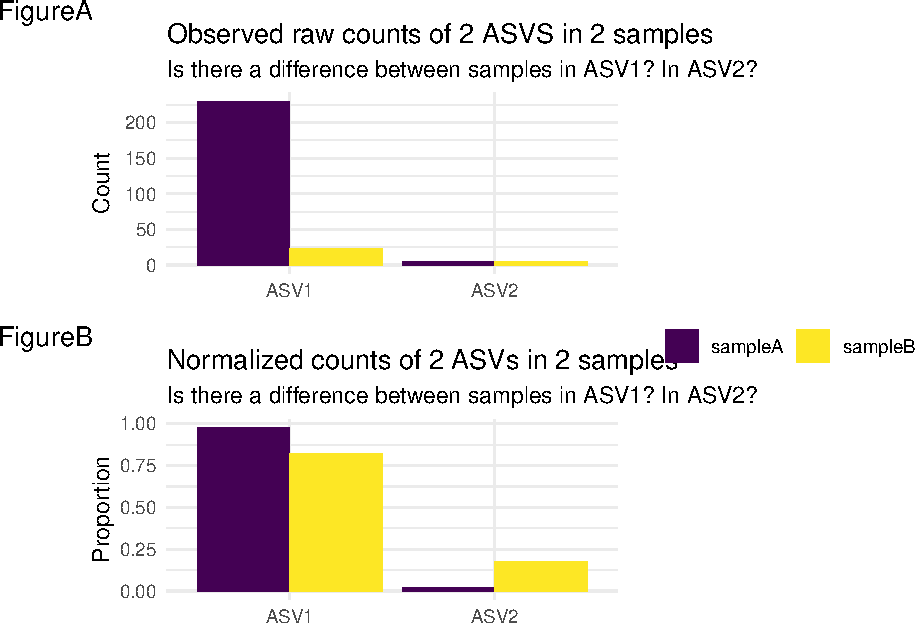
\includegraphics{MB_normalization_review_files/figure-latex/demo_normalization_importance-1.pdf}

Normalization for microbiome data often refers to standardizing sequencing depth across samples. One common approach to this is a scaling-based approach, where a scaling factor is calculated for every sample and the counts for each taxon are divided by the scaling factor for that sample. Figure B shows the same data as figure A, but where each sample has been transformed into proportions by dividing by the total counts for each sample. The difference in \texttt{ASV1} between samples appears much smaller. However, now there appears to be a difference in \texttt{ASV2}, even though the counts were originally the same. This is because in sample B \texttt{ASV1} consists of a higher proportion of the total count than in sample A.

This demonstrates the importance of normalization, but also the artifacts that can occur depending on the method.

\hypertarget{the-compositional-nature-of-microbiome-data}{%
\section{The compositional nature of microbiome data}\label{the-compositional-nature-of-microbiome-data}}

Microbiome data are inherently compositional. The counts of the collection of taxa that make up each sample are constrained by the total sum, or sequencing depth for that sample. This means that the count of each sampled taxon is a portion of a larger whole. Each observed taxon is not independent. As we saw in the above example, before normalization, \texttt{ASV2} was equal between samples. After converting to proportions, \texttt{ASV2} no longer appears equal. If there is a difference between two samples it is unclear if that difference is because of a true difference in that taxon or if that taxon is changing because of differences in another taxon. Numerous traditional statistical methods rely on an independence assumption, which is not met with microbiome data. This can lead to spurious correlations that exist only because of the compositional nature and not any true signal.

With library size as the sum constraint for each sample, if we know in a biological system that after an event occurs (treatment), the red taxon decreases, this will change the composition of the sampled blue taxon regardless of its change or lack thereof in the underlying population.

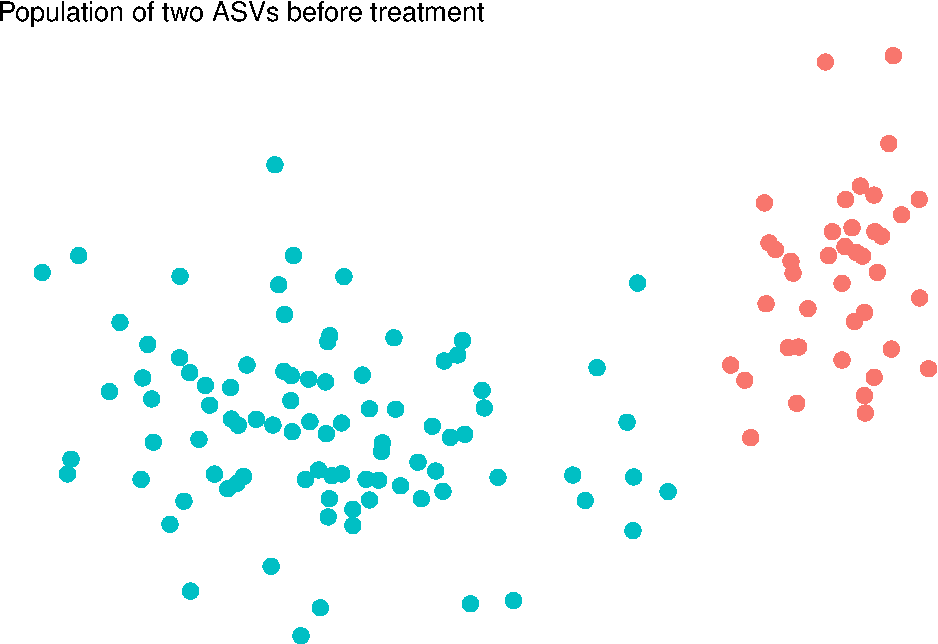
\includegraphics{MB_normalization_review_files/figure-latex/compositional-plot-1.pdf}

Consider again two samples consisting of red and blue points. We can think of the samples as before and after treatment. In the second plot, the number of red dots in the population and in the observed sample has decreased, but the blue remains the same.

\begin{table}

\caption{\label{tab:compositional-tibble}Counts of sampled red and blue taxa before and after}
\centering
\begin{tabular}[t]{l|r|r}
\hline
Sample & blue & red\\
\hline
Before & 10 & 20\\
\hline
After & 10 & 4\\
\hline
\end{tabular}
\end{table}

\begin{table}

\caption{\label{tab:compositional-tibble}Proportions of sampled red and blue taxa before and after}
\centering
\begin{tabular}[t]{l|r|r}
\hline
Sample & blue & red\\
\hline
Before & 0.2857143 & 0.6666667\\
\hline
After & 0.7142857 & 0.3333333\\
\hline
\end{tabular}
\end{table}

This observed increase in the proportion of blue is due to the compositional nature of the sampled points, and not any true difference in the blue population.

\hypertarget{log-ratio-methods}{%
\subsection{Log ratio methods}\label{log-ratio-methods}}

The log-ratio based methodology developed by Aitchison in the 1980s is useful for analyzing compositional data \citep{aitchison1982}. Taking the logarithm of ratios can be an appropriate transformation for compositional data, so standard statistical tests can be appropriate again. This transformation removes the issue of standardizing/normalizing different sampling depths. The sampling depth for a given sample will not distort the biological covariance or correlation structure.

This log-ratio method has a drawback, which is the decision of how to define the denominator. One approach to this problem is to use one sample as the reference. This sample should be `representative'. The log-ratio transformation is then the ratio of every other taxon to that representative sample. Of course, knowledge of what makes a sample representative is hard to come by and often unknown, and subsequent results can be affected by this choice. This method is frequently called the additive log-ratio approach (alr). The alternative approach is to use the data to create a pseudo-reference sample. This pseudo-reference sample is the geometric mean of the counts of all taxa. This is called the centered log-ratio method.

While promising, these log-ratio methods have drawbacks in practice. Microbiome data are often incredibly sparse, with up to 80-90\% of count matrices containing zero counts. For ratio transformations, if we have sparse data, the geometric mean can be zero. Then the ratio is undefined, and further, so is the logarithm of zero count taxa.

One solution to this is adding a small pseudo count to every element in the data. This removes problems occurring from having zero counts in the data, but there is not a clear best choice of what pseudo count to use, and it the choice can impact downstream results.

\hypertarget{importing-data}{%
\chapter{Importing Data}\label{importing-data}}

There are multiple publicly available pre-compiled microbiome data sets. These data sets begin after the bioinformatics pipeline and are matrices of counts of OTUs per sample. These data sets can exist as \texttt{phyloseq} objects, a popular R package for microbiome analysis \citep{mcmurdie2013}, or as separate tables of counts and metadata.

\hypertarget{global-patterns}{%
\section{Global Patterns}\label{global-patterns}}

The Global Patterns dataset \citep{caporaso2011} is an available dataset in the \texttt{phyloseq} package. These data contain samples from 25 different environmental samples and mock communities. The sampling depth of these samples averages 3.1 million total counts. We will use this dataset to work through the different normalization methods.

The following lines load the relevant packages and data.

\begin{Shaded}
\begin{Highlighting}[]
\KeywordTok{library}\NormalTok{(tidyverse)}
\KeywordTok{library}\NormalTok{(phyloseq)}
\end{Highlighting}
\end{Shaded}

\begin{verbatim}
## 
## Attaching package: 'phyloseq'
\end{verbatim}

\begin{verbatim}
## The following object is masked from 'package:SummarizedExperiment':
## 
##     distance
\end{verbatim}

\begin{verbatim}
## The following object is masked from 'package:Biobase':
## 
##     sampleNames
\end{verbatim}

\begin{verbatim}
## The following object is masked from 'package:GenomicRanges':
## 
##     distance
\end{verbatim}

\begin{verbatim}
## The following object is masked from 'package:IRanges':
## 
##     distance
\end{verbatim}

\begin{Shaded}
\begin{Highlighting}[]
\KeywordTok{data}\NormalTok{(}\StringTok{"GlobalPatterns"}\NormalTok{)}
\CommentTok{\# examine phyloseq object }
\NormalTok{GlobalPatterns}
\end{Highlighting}
\end{Shaded}

\begin{verbatim}
## phyloseq-class experiment-level object
## otu_table()   OTU Table:         [ 19216 taxa and 26 samples ]
## sample_data() Sample Data:       [ 26 samples by 7 sample variables ]
## tax_table()   Taxonomy Table:    [ 19216 taxa by 7 taxonomic ranks ]
## phy_tree()    Phylogenetic Tree: [ 19216 tips and 19215 internal nodes ]
\end{verbatim}

\hypertarget{pre-processing-quality-control-and-filtering}{%
\section{Pre-processing Quality Control and Filtering}\label{pre-processing-quality-control-and-filtering}}

In addition to normalization, there are some steps we can perform that ideally remove technical artifacts from the sequencing process that only introduce noise.

These filtering steps commonly consist of filtering out samples with a low total read depth and filtering out taxa that are rarely abundant.

Let's create a filtered version of the Global Patterns dataset. Note that there are only 26 samples, and all have a large library size, so we will not filter out any samples here.

For taxa filtering, we will remove taxa that appear fewer than 5 times in more than half the samples.

\begin{Shaded}
\begin{Highlighting}[]
\CommentTok{\# Determine which taxa to remove}
\NormalTok{filter\_taxa \textless{}{-}}\StringTok{ }\KeywordTok{genefilter\_sample}\NormalTok{(GlobalPatterns,}
                                 \KeywordTok{filterfun\_sample}\NormalTok{(}\ControlFlowTok{function}\NormalTok{(x) x }\OperatorTok{\textgreater{}}\StringTok{ }\DecValTok{5}\NormalTok{),}
                                 \DataTypeTok{A=}\FloatTok{0.5}\OperatorTok{*}\KeywordTok{nsamples}\NormalTok{(GlobalPatterns))}
\CommentTok{\# Remove those taxa from the GlobalPatterns dataset}
\CommentTok{\# Save as an object with the un{-}normalized counts}
\NormalTok{gp\_raw \textless{}{-}}\StringTok{ }\KeywordTok{prune\_taxa}\NormalTok{(filter\_taxa, GlobalPatterns)}
\NormalTok{gp\_raw}
\end{Highlighting}
\end{Shaded}

\begin{verbatim}
## phyloseq-class experiment-level object
## otu_table()   OTU Table:         [ 219 taxa and 26 samples ]
## sample_data() Sample Data:       [ 26 samples by 7 sample variables ]
## tax_table()   Taxonomy Table:    [ 219 taxa by 7 taxonomic ranks ]
## phy_tree()    Phylogenetic Tree: [ 219 tips and 218 internal nodes ]
\end{verbatim}

This decreases the number of taxa from 19216 to 219. This is not surprising, because this dataset contains samples from widely different locations (gut, soil, etc), and few taxa are shared among all samples and locations. One potential problem with this approach is the widely different locations, so it is possible that the remaining taxa could be some technical artifact, or could be a general `core' set of taxa shared across the disparate environments.

Additionally, let us save the total sampling depth as the variable \texttt{depth} in the metadata for the Global Patterns dataset.

\begin{Shaded}
\begin{Highlighting}[]
\NormalTok{gp\_raw}\OperatorTok{@}\NormalTok{sam\_data}\OperatorTok{$}\NormalTok{depth \textless{}{-}}\StringTok{ }\KeywordTok{sample\_sums}\NormalTok{(gp\_raw)}
\end{Highlighting}
\end{Shaded}

We can visualize technical artifacts of sapling depth is by looking at principal coordinates plots using the Bray-Curtis dissimilarity, coloring by sampling depth too see how much variation can be explained by the original sampling depth.

\begin{Shaded}
\begin{Highlighting}[]
\NormalTok{gp\_raw\_dist \textless{}{-}}\StringTok{ }\NormalTok{phyloseq}\OperatorTok{::}\KeywordTok{ordinate}\NormalTok{(gp\_raw, }\StringTok{"PCoA"}\NormalTok{, }\StringTok{"bray"}\NormalTok{)}
\KeywordTok{plot\_ordination}\NormalTok{(gp\_raw,}
\NormalTok{                gp\_raw\_dist,}
                \DataTypeTok{color =} \StringTok{"depth"}\NormalTok{, }
                \DataTypeTok{title =} \StringTok{"PCoA on Raw counts"}\NormalTok{)}
\end{Highlighting}
\end{Shaded}

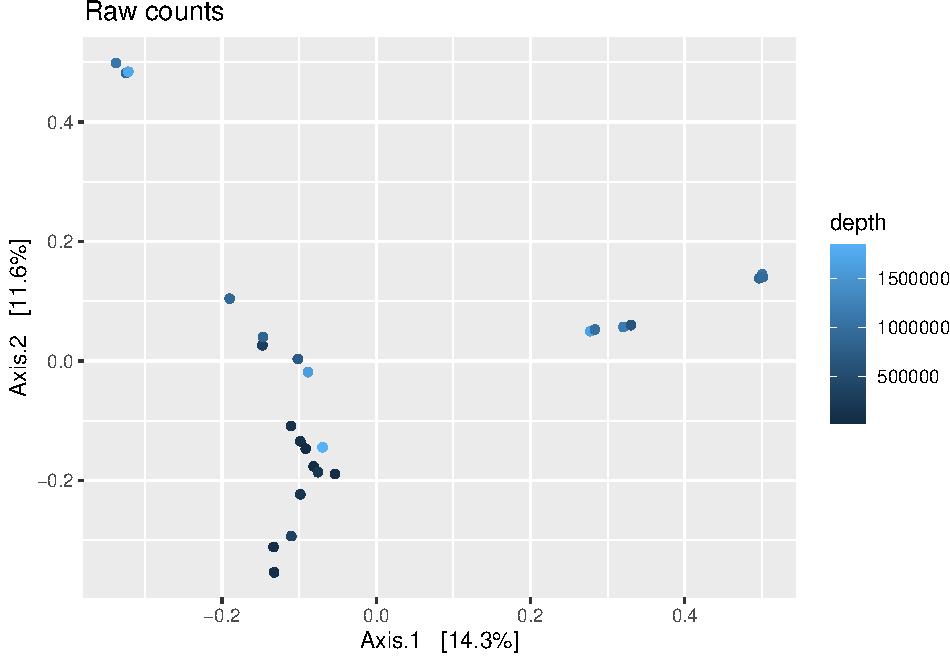
\includegraphics{MB_normalization_review_files/figure-latex/rare_depth_ordcolor-1.pdf}

We don't see any extreme patterns with sampling depth, but this might additionally be due to the differences in different locations might have different sampling depths. This comparison might be more interesting when we only have one location we are sampling from.

\hypertarget{total-sum-scaling-tss}{%
\chapter{Total Sum scaling (TSS)}\label{total-sum-scaling-tss}}

\hypertarget{about-tss}{%
\section{About TSS}\label{about-tss}}

The first method described is Total Sum Scaling (TSS). This method is also referred to as Total Count (TC), converting into proportions, or relative abundance. This is a scaling method to normalize the different library sizes across samples. For every entry in the count matrix, we scale by the total read depth of that sample. This converts the counts into the proportion of abundance present in each given sample.

Though a more straightforward method, TSS normalization is not without its drawbacks. In microbiome data, it is common to have numerous low or zero-count observations, and that only a few most common OTUs contribute to the majority of the total sum of the sampling depth. These high-count, frequent, taxa could be an artifact of the sequencing step, where high abundance observations are preferentially sampled. Using these large counts can dominate the scaling factor for each sample. As seen below, we see that the scaling factor for each sample is completely dominated by \texttt{ASV1}, if that one taxon were not included in the sample, the scaling factor would be widely different.

\begin{tabular}{l|r|r|r|r|r|r}
\hline
Sample & ASV1 & ASV2 & ASV3 & ASV4 & TSS Scaling Factor & Scaling factor w/o ASV1\\
\hline
Sample A & 10314 & 34 & 8 & 12 & 10368 & 54\\
\hline
Sample B & 824 & 23 & 13 & 20 & 880 & 56\\
\hline
\end{tabular}

Because this method does not account for the preferential sequencing over-abundance of \texttt{ASV1} it is possible to see an increase in false positives. However, this is a widely used method, and one of the few normalization methods that completely accounts for differing library sizes, which can be an important consideration depending on the analysis goal. Community level-analysis for example can be library-size dependent (ordination, some dissimiliarity measures).

\hypertarget{tss-implementation}{%
\section{TSS Implementation}\label{tss-implementation}}

Here, we provide a function that will normalize a \texttt{phyloseq} object by Total Sum Scaling. We have the option of keeping the result as proportions (having values 0-1), or transforming to an equal sequencing depth so the results are counts per million.

\begin{Shaded}
\begin{Highlighting}[]
\NormalTok{norm\_TSS \textless{}{-}}\StringTok{ }\ControlFlowTok{function}\NormalTok{(ps, }\DataTypeTok{keep\_prop =}\NormalTok{ F)\{}
    \CommentTok{\# keep as proportions or convert to counts per million?}
\NormalTok{    scale \textless{}{-}}\StringTok{ }\KeywordTok{ifelse}\NormalTok{(keep\_prop, }\DecValTok{1}\NormalTok{, }\FloatTok{1e6}\NormalTok{)}
    \CommentTok{\# TSS function}
\NormalTok{    ps\_normed \textless{}{-}}\StringTok{ }\NormalTok{phyloseq}\OperatorTok{::}\KeywordTok{transform\_sample\_counts}\NormalTok{(ps, }\ControlFlowTok{function}\NormalTok{(x) x }\OperatorTok{*}\StringTok{ }\NormalTok{scale }\OperatorTok{/}\StringTok{ }\KeywordTok{sum}\NormalTok{(x))}
    \KeywordTok{return}\NormalTok{(ps\_normed)}
\NormalTok{\}}
\end{Highlighting}
\end{Shaded}

\hypertarget{tss-on-global-patterns}{%
\section{TSS on Global Patterns}\label{tss-on-global-patterns}}

Using the above function, we apply this normalization to the Global Patterns data.

\begin{Shaded}
\begin{Highlighting}[]
\NormalTok{gp\_tss \textless{}{-}}\StringTok{ }\KeywordTok{norm\_TSS}\NormalTok{(gp\_raw)}
\CommentTok{\# rename the depth as the scaling factor }
\KeywordTok{sample\_data}\NormalTok{(gp\_tss)}\OperatorTok{$}\NormalTok{scaling\_factor \textless{}{-}}\StringTok{ }\KeywordTok{sample\_data}\NormalTok{(gp\_tss)}\OperatorTok{$}\NormalTok{depth}
\end{Highlighting}
\end{Shaded}

To see the differences between the un-normalized, raw data, and the TSS transformed normalized data, one possible way is to look at ordination plots. Microbiome data are high dimensional, so visualization directly of the data is difficult. Here, let us examine the principal coordinates plot using the Bray-Curtis dissimilarity.

First calculate the distance matrices, using the \texttt{phyloseq} function \texttt{ordinate()}

\begin{Shaded}
\begin{Highlighting}[]
\NormalTok{gp\_raw\_dist \textless{}{-}}\StringTok{ }\NormalTok{phyloseq}\OperatorTok{::}\KeywordTok{ordinate}\NormalTok{(gp\_raw, }\StringTok{"PCoA"}\NormalTok{, }\StringTok{"bray"}\NormalTok{)}
\NormalTok{gp\_tss\_dist \textless{}{-}}\StringTok{ }\NormalTok{phyloseq}\OperatorTok{::}\KeywordTok{ordinate}\NormalTok{(gp\_tss, }\StringTok{"PCoA"}\NormalTok{, }\StringTok{"bray"}\NormalTok{)}
\end{Highlighting}
\end{Shaded}

Now plot the two ordinations. Even before normalization, the different communities are clearly clustered.

(Note to self: perhaps choose a different dataset to use for walk-through, currently using Global Patterns since it is small and quick for computations, but harder to see differences.)

\begin{Shaded}
\begin{Highlighting}[]
\KeywordTok{plot\_ordination}\NormalTok{(gp\_raw, gp\_raw\_dist, }\DataTypeTok{color =} \StringTok{"SampleType"}\NormalTok{, }
                \DataTypeTok{title =} \StringTok{"PCoA on Raw Counts"}\NormalTok{) }\OperatorTok{+}\StringTok{ }
\KeywordTok{plot\_ordination}\NormalTok{(gp\_tss, gp\_tss\_dist, }\DataTypeTok{color =} \StringTok{"SampleType"}\NormalTok{, }
                \DataTypeTok{title =} \StringTok{"PCoA on TSS normalized counts"}\NormalTok{) }\OperatorTok{+}
\StringTok{  }\KeywordTok{plot\_layout}\NormalTok{(}\DataTypeTok{guides =} \StringTok{\textquotesingle{}collect\textquotesingle{}}\NormalTok{)}
\end{Highlighting}
\end{Shaded}

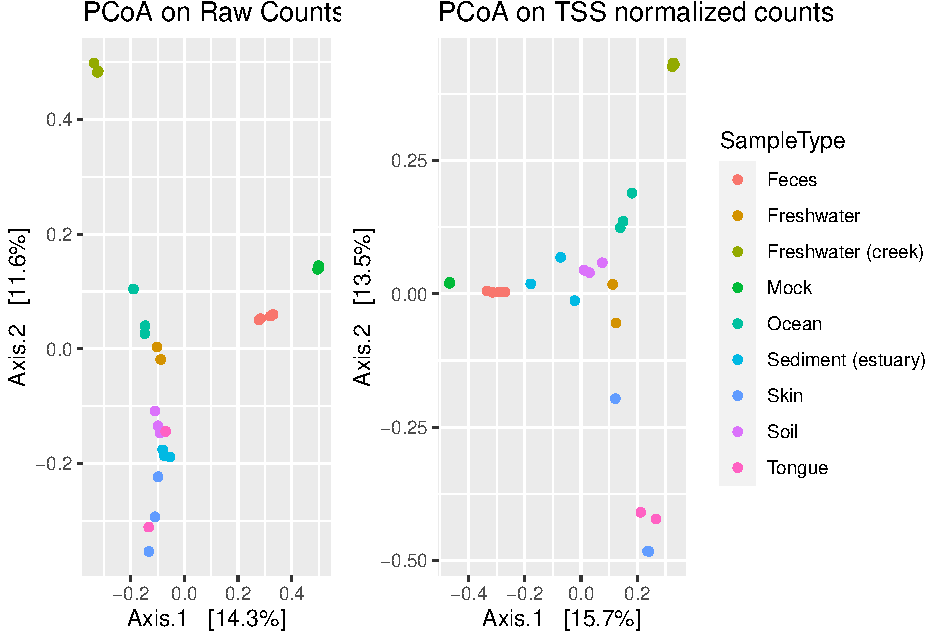
\includegraphics{MB_normalization_review_files/figure-latex/plot_ordinate_tss-1.pdf}

We can also compare the values of the distance matrices before and after normalization to see how the normalization method is impacting different types of points.

\begin{Shaded}
\begin{Highlighting}[]
\CommentTok{\# Function to visualize potential differences and changes after normalization methods}
\NormalTok{plot\_norm\_changes \textless{}{-}}\StringTok{ }\ControlFlowTok{function}\NormalTok{(data\_norm, data\_raw, }\DataTypeTok{dist\_method =} \StringTok{"bray"}\NormalTok{, }\DataTypeTok{x\_lab =} \StringTok{"raw"}\NormalTok{, }\DataTypeTok{y\_lab =} \StringTok{"norm"}\NormalTok{, }\DataTypeTok{title =} \StringTok{"Plot title"}\NormalTok{)\{}
    \CommentTok{\# calculate the Bray{-}Cutris distance matrix for the raw data, the normalized data, }
    \CommentTok{\# and calculate the pairwise difference between the original library sizes between samples}
\NormalTok{    plot \textless{}{-}}\StringTok{ }\KeywordTok{data.frame}\NormalTok{(}\DataTypeTok{raw =} \KeywordTok{as.numeric}\NormalTok{(phyloseq}\OperatorTok{::}\KeywordTok{distance}\NormalTok{(data\_raw, dist\_method)), }
                       \DataTypeTok{norm =} \KeywordTok{as.numeric}\NormalTok{(phyloseq}\OperatorTok{::}\KeywordTok{distance}\NormalTok{(data\_norm, dist\_method)), }
                       \DataTypeTok{diff =} \KeywordTok{as.numeric}\NormalTok{(}\KeywordTok{dist}\NormalTok{(}\KeywordTok{get\_variable}\NormalTok{(data\_raw, }\StringTok{"depth"}\NormalTok{)))) }\OperatorTok{\%\textgreater{}\%}\StringTok{ }
\StringTok{    }\KeywordTok{ggplot}\NormalTok{(}\KeywordTok{aes}\NormalTok{(}\DataTypeTok{x =}\NormalTok{ raw, }\DataTypeTok{y =}\NormalTok{ norm, }\DataTypeTok{color =}\NormalTok{ diff)) }\OperatorTok{+}\StringTok{ }
\StringTok{        }\KeywordTok{geom\_point}\NormalTok{() }\OperatorTok{+}\StringTok{ }
\StringTok{        }\KeywordTok{geom\_abline}\NormalTok{() }\OperatorTok{+}\StringTok{ }
\StringTok{        }\KeywordTok{ggtitle}\NormalTok{(title) }\OperatorTok{+}
\StringTok{        }\KeywordTok{xlab}\NormalTok{(x\_lab) }\OperatorTok{+}\StringTok{ }\KeywordTok{ylab}\NormalTok{(y\_lab) }\OperatorTok{+}
\StringTok{        }\KeywordTok{labs}\NormalTok{(}\DataTypeTok{color =} \StringTok{"Pairwise difference in sampling depth"}\NormalTok{)}\OperatorTok{+}
\StringTok{      }\KeywordTok{xlim}\NormalTok{(}\KeywordTok{c}\NormalTok{(}\DecValTok{0}\NormalTok{,}\DecValTok{1}\NormalTok{)) }\OperatorTok{+}\StringTok{ }\KeywordTok{ylim}\NormalTok{(}\KeywordTok{c}\NormalTok{(}\DecValTok{0}\NormalTok{,}\DecValTok{1}\NormalTok{))}
    \KeywordTok{return}\NormalTok{(plot)}
\NormalTok{\}}

\KeywordTok{plot\_norm\_changes}\NormalTok{(gp\_tss, gp\_raw,}
                  \DataTypeTok{x\_lab =} \StringTok{"Raw counts"}\NormalTok{, }\DataTypeTok{y\_lab =} \StringTok{"TSS props"}\NormalTok{, }
                  \DataTypeTok{title =} \StringTok{"Distance metric comparision between Raw counts and TSS normalized counts "}\NormalTok{)}
\end{Highlighting}
\end{Shaded}

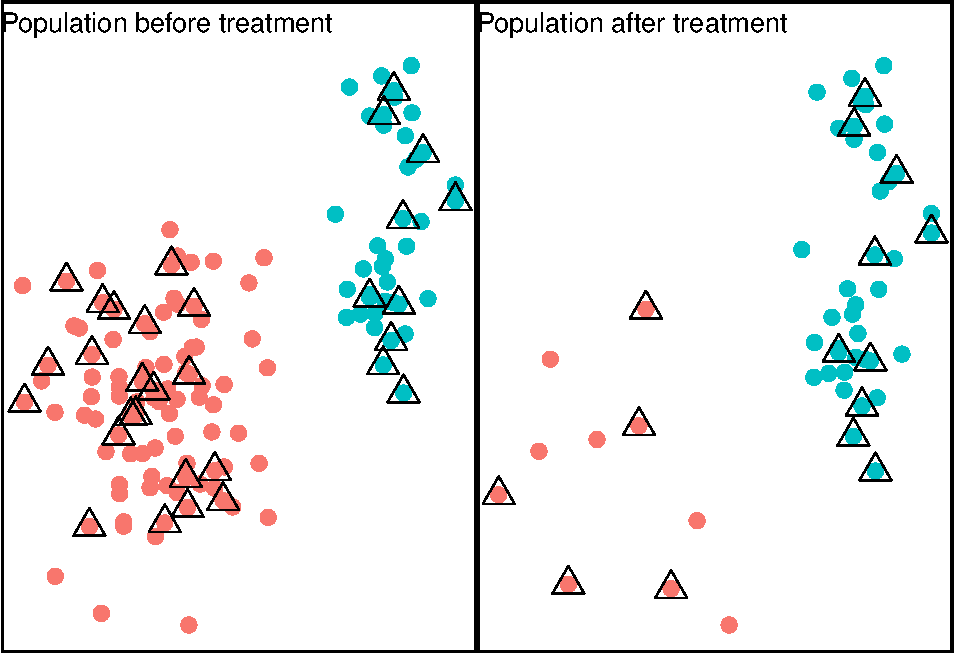
\includegraphics{MB_normalization_review_files/figure-latex/unnamed-chunk-3-1.pdf}

Points below the line are pairs of samples that are marked as more similar after normalization. Points above the line are marked as more different after normalization. Values closer to 1 are `more different'. Unsurprisingly, pairs that had larger original differences in sampling depth were marked as more different on the raw, un-normalized data, and became marked as more similar after TSS normalization.

\hypertarget{rarefying}{%
\chapter{Rarefying}\label{rarefying}}

\hypertarget{about-rarefying}{%
\section{About Rarefying}\label{about-rarefying}}

Rarefying is another common normalization technique that standardizes the library size across samples that was originally used in ecology. This method standardizes the read depth across all samples. To perform this method we first choose a minimum library size. Looking at rarefaction/collectors curves, or using a certain percentile can guide choosing this cutoff. Then all samples that have a read depth below this cutoff are discarded. Thus this method has a built-in filtering step. Next, we sample without replacement of the size of the chosen cutoff. It can be a standalone method or combined with other methods and transformations.

This is a very commonly used method, but it has also been criticized \citep{mcmurdie2014}. First of all, it throws away valid data, and this results in a loss of power and an increase in false positives. Rare taxa can be removed in this approach too. It is however encouraged when we have widely different library sizes as it can lower the false discovery rate \citep{weiss2017}, and has also been shown to perform well in community-level analysis \citep{mcknight2019}, as it completely standardizes the read count depth, and some methods are sensitive to differences in read count. Rarefying has been shown to separate by biological signal in ordination methods based on presence/absence.

\hypertarget{rarefying-implementation}{%
\section{Rarefying implementation}\label{rarefying-implementation}}

The following function returns a rarefied \texttt{phyloseq} object. We can either pass in the minimum sampling depth as a second argument, or use the default minimum depth of the samples.

\begin{Shaded}
\begin{Highlighting}[]
\NormalTok{norm\_rarefy \textless{}{-}}\StringTok{ }\ControlFlowTok{function}\NormalTok{(phyloseq, }\DataTypeTok{depth =} \KeywordTok{min}\NormalTok{(}\KeywordTok{sample\_sums}\NormalTok{(phyloseq)))\{}
    \KeywordTok{return}\NormalTok{(phyloseq}\OperatorTok{::}\KeywordTok{rarefy\_even\_depth}\NormalTok{(phyloseq,}\DataTypeTok{sample.size =}\NormalTok{ depth))}
\NormalTok{\}}
\end{Highlighting}
\end{Shaded}

\hypertarget{rarefying-on-global-patterns}{%
\section{Rarefying on Global Patterns}\label{rarefying-on-global-patterns}}

We use the above function to rarefy the Global Patterns data. The first difficulty is choosing a minimum sampling depth. The Global Patterns dataset already has a very high sampling depth for all samples, so we will chose the lowest as the minimum depth to rarefy to.Since we chose the minimum sampling depth, no samples have been dropped. In data sets where we have low sampling depth there is a balance between how many samples to drop and how low to set the minimum depth to.

\begin{Shaded}
\begin{Highlighting}[]
\NormalTok{gp\_rare \textless{}{-}}\StringTok{ }\KeywordTok{norm\_rarefy}\NormalTok{(gp\_raw)}
\end{Highlighting}
\end{Shaded}

\begin{verbatim}
## You set `rngseed` to FALSE. Make sure you've set & recorded
##  the random seed of your session for reproducibility.
## See `?set.seed`
\end{verbatim}

\begin{verbatim}
## ...
\end{verbatim}

We can check that indeed all samples now have the same sampling depth, which is 15905. Note that the highest sampling depth in this dataset was almost 2 million, so we have discarded a lot of data to reduce to 15905.

\begin{Shaded}
\begin{Highlighting}[]
\KeywordTok{max}\NormalTok{(}\KeywordTok{sample\_sums}\NormalTok{(gp\_raw))}
\end{Highlighting}
\end{Shaded}

\begin{verbatim}
## [1] 1842380
\end{verbatim}

\begin{Shaded}
\begin{Highlighting}[]
\KeywordTok{sample\_sums}\NormalTok{(gp\_rare)}
\end{Highlighting}
\end{Shaded}

\begin{verbatim}
##      CL3      CC1      SV1  M31Fcsw  M11Fcsw  M31Plmr  M11Plmr  F21Plmr 
##    15905    15905    15905    15905    15905    15905    15905    15905 
##  M31Tong  M11Tong LMEpi24M SLEpi20M   AQC1cm   AQC4cm   AQC7cm      NP2 
##    15905    15905    15905    15905    15905    15905    15905    15905 
##      NP3      NP5  TRRsed1  TRRsed2  TRRsed3     TS28     TS29    Even1 
##    15905    15905    15905    15905    15905    15905    15905    15905 
##    Even2    Even3 
##    15905    15905
\end{verbatim}

We can again compare the PCoA plots between rarefied and raw counts, coloring by sample type to view clusters.

\begin{Shaded}
\begin{Highlighting}[]
\KeywordTok{plot\_ordination}\NormalTok{(gp\_raw,}
\NormalTok{                phyloseq}\OperatorTok{::}\KeywordTok{ordinate}\NormalTok{(gp\_raw, }\StringTok{"PCoA"}\NormalTok{, }\StringTok{"bray"}\NormalTok{),}
                \DataTypeTok{color =} \StringTok{"SampleType"}\NormalTok{, }
                \DataTypeTok{title =} \StringTok{"PCoA on Raw counts"}\NormalTok{) }\OperatorTok{+}
\KeywordTok{plot\_ordination}\NormalTok{(gp\_rare,}
\NormalTok{                phyloseq}\OperatorTok{::}\KeywordTok{ordinate}\NormalTok{(gp\_rare, }\StringTok{"PCoA"}\NormalTok{, }\StringTok{"bray"}\NormalTok{),}
                \DataTypeTok{color =} \StringTok{"SampleType"}\NormalTok{, }
                \DataTypeTok{title =} \StringTok{"PCoA on Rarefied counts"}\NormalTok{)}\OperatorTok{+}
\StringTok{  }\KeywordTok{plot\_layout}\NormalTok{(}\DataTypeTok{guides =} \StringTok{\textquotesingle{}collect\textquotesingle{}}\NormalTok{)}
\end{Highlighting}
\end{Shaded}

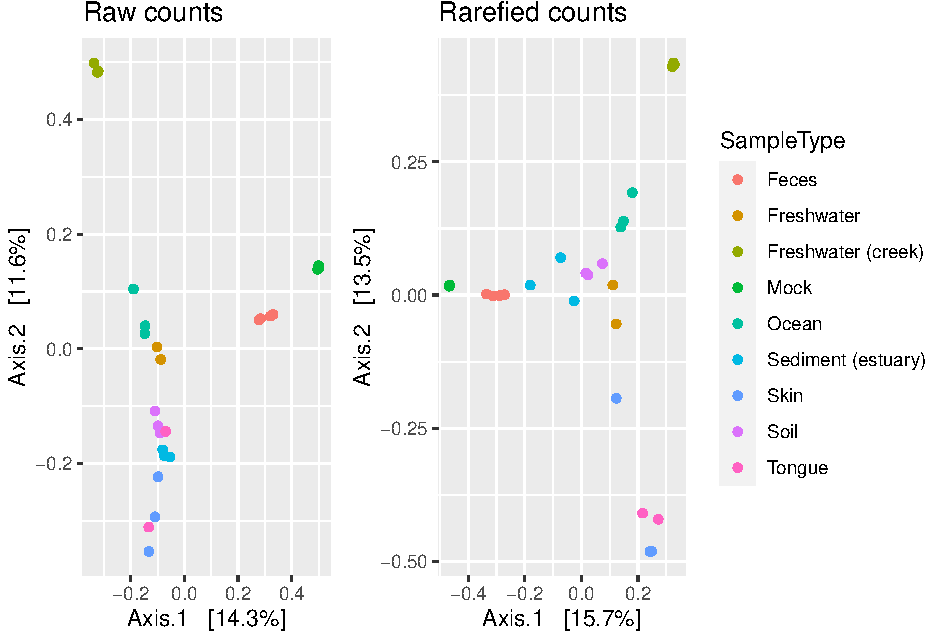
\includegraphics{MB_normalization_review_files/figure-latex/rare_ordination-1.pdf}

Now examine how the distance matrices change before/after normalization. We see a similar pattern to TSS when distance matrices calculated from rarefied counts are compared to those from the raw counts.

\begin{Shaded}
\begin{Highlighting}[]
\CommentTok{\# Identify any samples filtered in rarefying process }
\NormalTok{rare\_samples \textless{}{-}}\StringTok{ }\KeywordTok{sample\_names}\NormalTok{(gp\_rare)}
\NormalTok{gp\_raw\_match \textless{}{-}}\StringTok{ }\KeywordTok{prune\_samples}\NormalTok{(rare\_samples, gp\_raw)}
\KeywordTok{plot\_norm\_changes}\NormalTok{(gp\_rare, gp\_raw\_match,}
                  \DataTypeTok{x\_lab =} \StringTok{"Raw counts"}\NormalTok{, }\DataTypeTok{y\_lab =} \StringTok{"Rarefied counts"}\NormalTok{, }
                  \DataTypeTok{title =} \StringTok{"Distance metric comparision between Raw counts and Rarefied counts "}\NormalTok{)}
\end{Highlighting}
\end{Shaded}

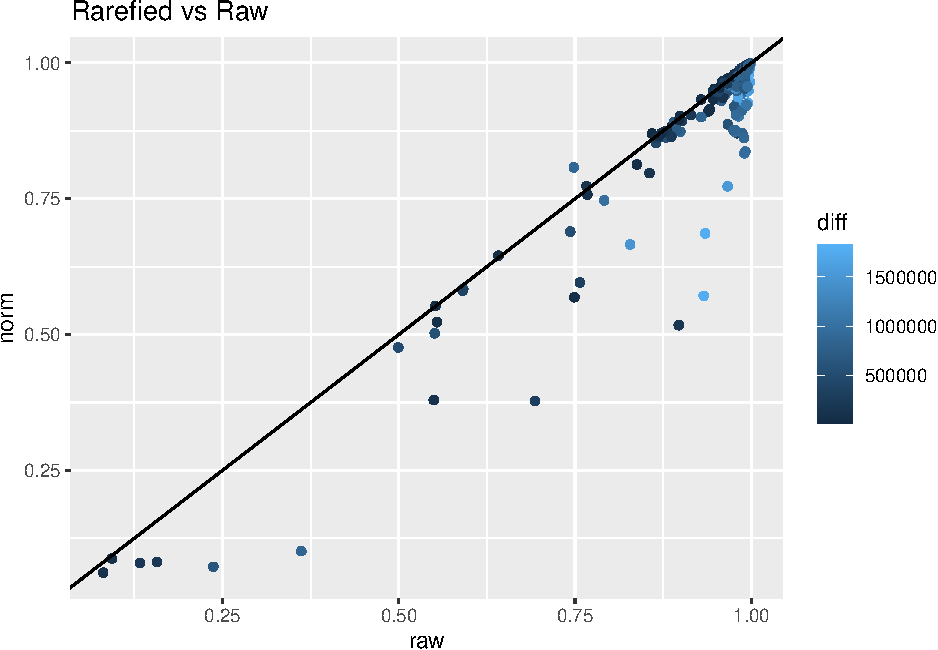
\includegraphics{MB_normalization_review_files/figure-latex/rare_plot_ordination-1.pdf}

\begin{Shaded}
\begin{Highlighting}[]
\CommentTok{\#\# Compare to tss}
\NormalTok{gp\_tss\_match \textless{}{-}}\StringTok{ }\KeywordTok{norm\_TSS}\NormalTok{(gp\_raw\_match)}
\KeywordTok{plot\_norm\_changes}\NormalTok{(gp\_rare, gp\_tss,}
                  \DataTypeTok{x\_lab =} \StringTok{"TSS"}\NormalTok{, }\DataTypeTok{y\_lab =} \StringTok{"Rarefied"}\NormalTok{, }
                  \DataTypeTok{title =} \StringTok{"Distance metric comparision between TSS normalization and Rarefied counts "}\NormalTok{)}
\end{Highlighting}
\end{Shaded}

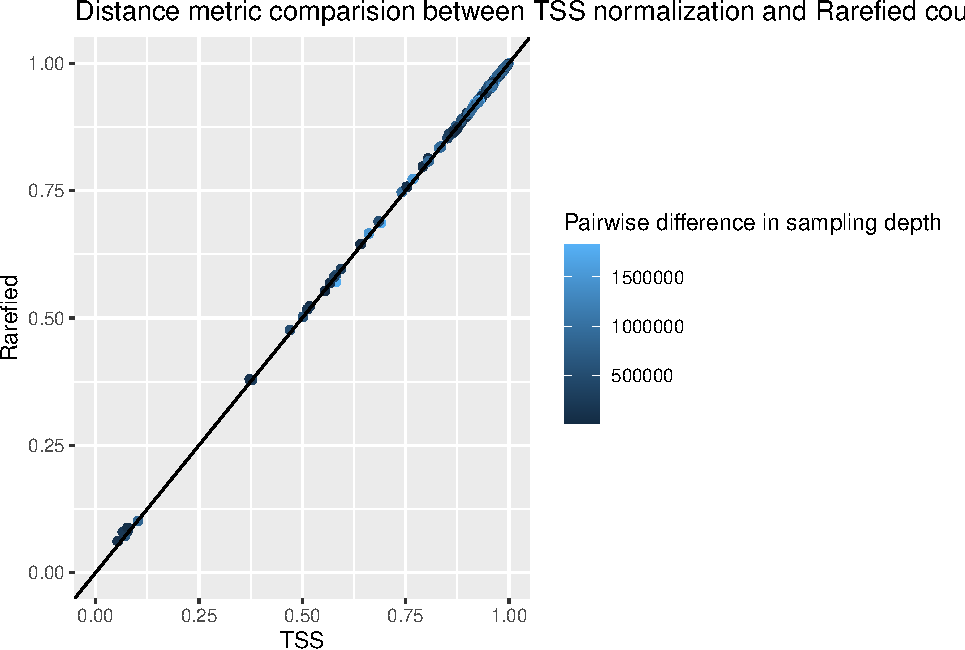
\includegraphics{MB_normalization_review_files/figure-latex/rare_plot_ordination-2.pdf}

\hypertarget{deseq}{%
\chapter{DESeq}\label{deseq}}

\hypertarget{about-deseq}{%
\section{About DESeq}\label{about-deseq}}

DESeq2 includes a normalization method for adjusting for differing library sizes across samples \citep{anders2010}. This method also can account for differences in library composition. This method has also been called MED, RLE, or DESeq in the literature.

DESeq2 first takes the natural logarithm of every entry in the count matrix. Due to this, all entries with zero will be set to negative infinity. Next, the row average is calculated (geometric average), so we have a vector of average counts for each taxon. Taking the log first should avoid undue influence by extreme outliers. All taxa with an average of infinity are removed. This step will remove all taxa with zero read count in one or more samples. This can be a problem in microbiome data. Next, we subtract the average log value from the log(counts), this gives a log ratio. This is equivalent to the ratio of the reads in each sample to the average across all samples. Next, we calculate the median of the log-ratios for each sample. These medians are converted to scaling factors for each sample by exponentiation. An extension of this method, denoted `poscounts', has been suggested, which instead of taking the geometric mean of the logged counts for each taxon, we take the n-th root of the product of the non-zero counts.

This method assumes that the taxon of median absolute abundance is not differentially abundant, which is more likely true for the RNA-Seq it was developed for, but may not be true for microbiome studies, especially when there are more study groups, or we are analyzing higher taxonomic levels.

An additional option can be used to perform a variance stabilizing transformation on the count matrix before normalizing with the above size factors. This method calculates a dispersion-mean relationship and then transforms the data. The result ideally is an abundance matrix that is approximately homoskedastic or constant variance across the range of mean values. The package also includes an option for a `rlog' transform, which they recommend over the variance stabilizing method in the case when there is a large difference in library sizes.

If differential abundance is of interest to calculate, DESeq uses a negative binomial distribution to model differential abundances. It is possible to provide the size factors calculated by another method to DESeq to perform differential analysis.

\hypertarget{deseq-implementation}{%
\section{DESeq Implementation}\label{deseq-implementation}}

Here we provide two normalization functions using DESeq methods. The first calculates the RLE normalization using the \texttt{poscounts} option for microbiome data. The second calculates the variance stabalizing transformation.

\begin{Shaded}
\begin{Highlighting}[]
\NormalTok{norm\_DESeq\_RLE\_poscounts \textless{}{-}}\StringTok{ }\ControlFlowTok{function}\NormalTok{(ps, }\DataTypeTok{group =} \DecValTok{1}\NormalTok{)\{}
  \KeywordTok{require}\NormalTok{(DESeq2, }\DataTypeTok{quietly =}\NormalTok{ T)}
    \CommentTok{\# keep arbitrary design for normalization }
    \CommentTok{\# Convert to DESeq object}
\NormalTok{    ps\_dds \textless{}{-}}\StringTok{ }\KeywordTok{phyloseq\_to\_deseq2}\NormalTok{(ps, }\OperatorTok{\textasciitilde{}}\DecValTok{1}\NormalTok{)}
    \CommentTok{\# Calculate the size factors (scaling)}
\NormalTok{    ps\_dds \textless{}{-}}\StringTok{ }\KeywordTok{estimateSizeFactors}\NormalTok{(ps\_dds, }\DataTypeTok{type =} \StringTok{"poscounts"}\NormalTok{)}
    \CommentTok{\# Extract counts}
\NormalTok{    counts \textless{}{-}}\StringTok{ }\NormalTok{DESeq2}\OperatorTok{::}\KeywordTok{counts}\NormalTok{(ps\_dds, }\DataTypeTok{normalized =}\NormalTok{ T)}
    \CommentTok{\# Convert back to phyloseq}
\NormalTok{    otu \textless{}{-}}\StringTok{ }\KeywordTok{otu\_table}\NormalTok{(counts, }\DataTypeTok{taxa\_are\_rows =}\NormalTok{ T)}
\NormalTok{    sam \textless{}{-}}\StringTok{ }\KeywordTok{access}\NormalTok{(ps, }\StringTok{"sam\_data"}\NormalTok{)}
\NormalTok{    sam}\OperatorTok{$}\NormalTok{scaling\_factor \textless{}{-}}\StringTok{ }\KeywordTok{sizeFactors}\NormalTok{(ps\_dds)}
\NormalTok{    tax \textless{}{-}}\StringTok{ }\KeywordTok{access}\NormalTok{(ps, }\StringTok{"tax\_table"}\NormalTok{)}
\NormalTok{    phy \textless{}{-}}\StringTok{ }\KeywordTok{access}\NormalTok{(ps, }\StringTok{"phy\_tree"}\NormalTok{)}
\NormalTok{    ps\_DESeq \textless{}{-}}\StringTok{ }\KeywordTok{phyloseq}\NormalTok{(otu,sam,tax,phy)}
    \KeywordTok{return}\NormalTok{(ps\_DESeq)}
\NormalTok{\}}



\NormalTok{norm\_DESeq\_vs \textless{}{-}}\StringTok{ }\ControlFlowTok{function}\NormalTok{(ps, }\DataTypeTok{group =} \DecValTok{1}\NormalTok{)\{}
  \KeywordTok{require}\NormalTok{(DESeq2, }\DataTypeTok{quietly =}\NormalTok{ T)}
\NormalTok{  ps\_dds \textless{}{-}}\StringTok{ }\KeywordTok{phyloseq\_to\_deseq2}\NormalTok{(ps, }\OperatorTok{\textasciitilde{}}\StringTok{ }\DecValTok{1}\NormalTok{)}
\NormalTok{  ps\_dds \textless{}{-}}\StringTok{ }\KeywordTok{estimateSizeFactors}\NormalTok{(ps\_dds, }\DataTypeTok{type =} \StringTok{"poscounts"}\NormalTok{)}
  \CommentTok{\# Variance transformation}
\NormalTok{  ps\_dds \textless{}{-}}\StringTok{ }\KeywordTok{estimateDispersions}\NormalTok{(ps\_dds)}
\NormalTok{  abund \textless{}{-}}\StringTok{ }\KeywordTok{getVarianceStabilizedData}\NormalTok{(ps\_dds)}
  \CommentTok{\# don’t allow deseq to return negative counts}
  \CommentTok{\# add the minimum count to all values}
  \CommentTok{\# another option is to replace negative counts with 0}
\NormalTok{  abund \textless{}{-}}\StringTok{ }\NormalTok{abund }\OperatorTok{+}\StringTok{ }\KeywordTok{abs}\NormalTok{(}\KeywordTok{min}\NormalTok{(abund)) }
\NormalTok{  otu \textless{}{-}}\StringTok{ }\KeywordTok{otu\_table}\NormalTok{(abund, }\DataTypeTok{taxa\_are\_rows =}\NormalTok{ T)}
\NormalTok{  sam \textless{}{-}}\StringTok{ }\KeywordTok{access}\NormalTok{(ps, }\StringTok{"sam\_data"}\NormalTok{)}
\NormalTok{  tax \textless{}{-}}\StringTok{ }\KeywordTok{access}\NormalTok{(ps, }\StringTok{"tax\_table"}\NormalTok{)}
\NormalTok{  phy \textless{}{-}}\StringTok{ }\KeywordTok{access}\NormalTok{(ps, }\StringTok{"phy\_tree"}\NormalTok{)}
\NormalTok{  ps\_DESeq \textless{}{-}}\StringTok{ }\KeywordTok{phyloseq}\NormalTok{(otu,sam,tax,phy)}
  \KeywordTok{return}\NormalTok{(ps\_DESeq)}
\NormalTok{\}}
\end{Highlighting}
\end{Shaded}

\hypertarget{deseq-on-global-patterns}{%
\section{DESeq on Global Patterns}\label{deseq-on-global-patterns}}

Perform DESeq RLE normalization as well as DESeq variance stabilized transformation on Global Patterns:

\begin{Shaded}
\begin{Highlighting}[]
\NormalTok{gp\_deseq\_rle \textless{}{-}}\StringTok{ }\KeywordTok{norm\_DESeq\_RLE\_poscounts}\NormalTok{(gp\_raw)}
\end{Highlighting}
\end{Shaded}

\begin{verbatim}
## converting counts to integer mode
\end{verbatim}

\begin{Shaded}
\begin{Highlighting}[]
\NormalTok{gp\_deseq\_vs \textless{}{-}}\StringTok{ }\KeywordTok{norm\_DESeq\_vs}\NormalTok{(gp\_raw)}
\end{Highlighting}
\end{Shaded}

\begin{verbatim}
## converting counts to integer mode
\end{verbatim}

\begin{verbatim}
## gene-wise dispersion estimates
\end{verbatim}

\begin{verbatim}
## mean-dispersion relationship
\end{verbatim}

\begin{verbatim}
## -- note: fitType='parametric', but the dispersion trend was not well captured by the
##    function: y = a/x + b, and a local regression fit was automatically substituted.
##    specify fitType='local' or 'mean' to avoid this message next time.
\end{verbatim}

\begin{verbatim}
## final dispersion estimates
\end{verbatim}

Examine principal coordinate plots between raw data and both DESeq normalized data.

\begin{Shaded}
\begin{Highlighting}[]
\CommentTok{\# First calculate distance matrices }
\NormalTok{gp\_rle\_dist \textless{}{-}}\StringTok{ }\NormalTok{phyloseq}\OperatorTok{::}\KeywordTok{ordinate}\NormalTok{(gp\_deseq\_rle, }\StringTok{"PCoA"}\NormalTok{, }\StringTok{"bray"}\NormalTok{) }
\NormalTok{gp\_vs\_dist \textless{}{-}}\StringTok{ }\NormalTok{phyloseq}\OperatorTok{::}\KeywordTok{ordinate}\NormalTok{(gp\_deseq\_vs, }\StringTok{"PCoA"}\NormalTok{, }\StringTok{"bray"}\NormalTok{) }

\CommentTok{\# Plot ordinations}
\KeywordTok{plot\_ordination}\NormalTok{(gp\_raw, gp\_raw\_dist, }\DataTypeTok{color =} \StringTok{"SampleType"}\NormalTok{, }\DataTypeTok{title =} \StringTok{"PCoA on Raw data"}\NormalTok{) }\OperatorTok{+}\StringTok{ }
\KeywordTok{plot\_ordination}\NormalTok{(gp\_deseq\_rle, gp\_rle\_dist, }\DataTypeTok{color =} \StringTok{"SampleType"}\NormalTok{, }\DataTypeTok{title =} \StringTok{"PCoA on RLE"}\NormalTok{) }\OperatorTok{+}
\KeywordTok{plot\_ordination}\NormalTok{(gp\_deseq\_vs, gp\_vs\_dist, }\DataTypeTok{color =} \StringTok{"SampleType"}\NormalTok{, }\DataTypeTok{title =} \StringTok{"PCoA on VST"}\NormalTok{) }\OperatorTok{+}\StringTok{ }
\StringTok{  }\KeywordTok{plot\_layout}\NormalTok{(}\DataTypeTok{guides =} \StringTok{\textquotesingle{}collect\textquotesingle{}}\NormalTok{)}
\end{Highlighting}
\end{Shaded}

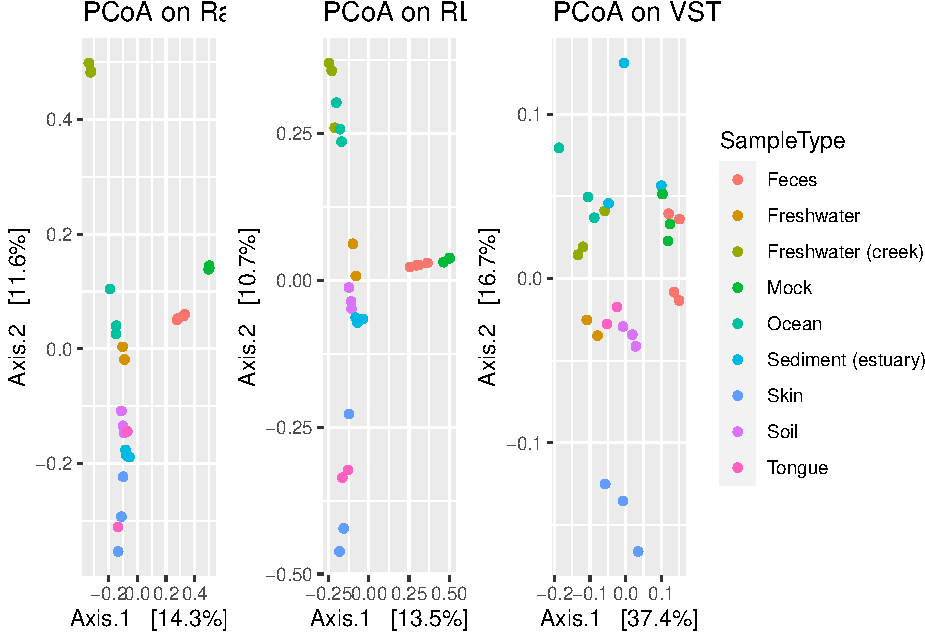
\includegraphics{MB_normalization_review_files/figure-latex/deseq-ordination-1.pdf}

See how dissimilarity matrices differ from raw counts and each DESeq transformation.

\begin{Shaded}
\begin{Highlighting}[]
\KeywordTok{plot\_norm\_changes}\NormalTok{(gp\_deseq\_rle, gp\_raw, }
                  \DataTypeTok{x\_lab =} \StringTok{"Raw"}\NormalTok{, }\DataTypeTok{y\_lab =} \StringTok{"RLE"}\NormalTok{, }
                  \DataTypeTok{title =} \StringTok{"Distance metric comparision between RLE normalization and Raw counts "}\NormalTok{) }\OperatorTok{/}\StringTok{ }
\KeywordTok{plot\_norm\_changes}\NormalTok{(gp\_deseq\_vs, gp\_raw, }
                  \DataTypeTok{x\_lab =} \StringTok{"Raw"}\NormalTok{, }\DataTypeTok{y\_lab =} \StringTok{"VST"}\NormalTok{, }
                  \DataTypeTok{title =} \StringTok{"Distance metric comparision between VST normalization and Raw counts "}\NormalTok{) }\OperatorTok{+}\StringTok{ }
\StringTok{  }\KeywordTok{plot\_layout}\NormalTok{(}\DataTypeTok{guides =} \StringTok{\textquotesingle{}collect\textquotesingle{}}\NormalTok{)}
\end{Highlighting}
\end{Shaded}

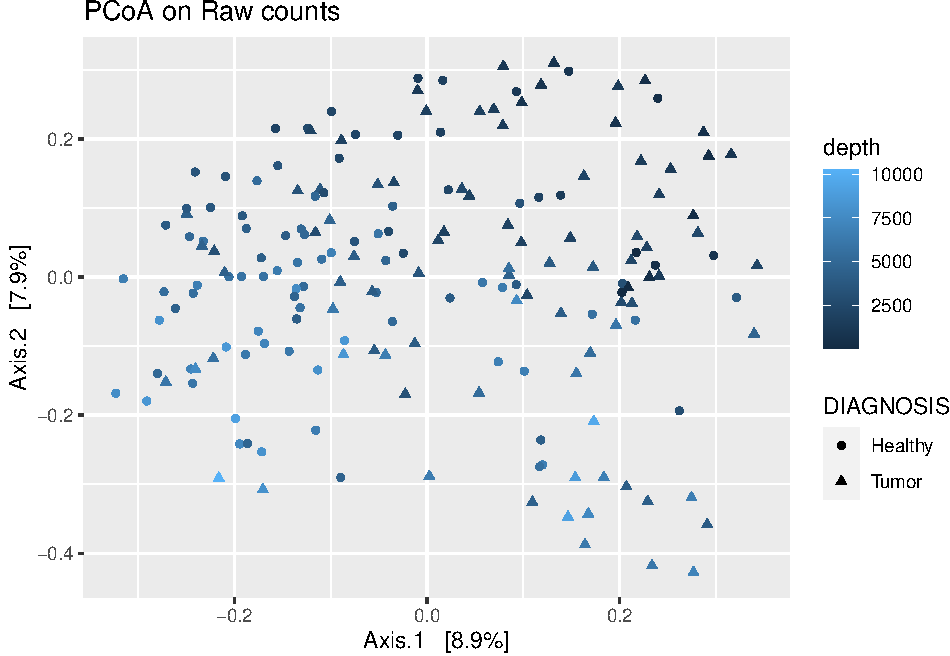
\includegraphics{MB_normalization_review_files/figure-latex/unnamed-chunk-7-1.pdf}

\hypertarget{tmm-edger}{%
\chapter{TMM (edgeR)}\label{tmm-edger}}

TMM (Trimmed median of m-values) is another method borrowed from RNA-Seq analysis, and implemented in \texttt{edgeR} \citep{robinson2010}. This method uses, or calculates a reference sample, and compares all other samples to the reference sample. The size factor is the mean of the log-ratios after excluding the highest count taxa and taxa with the largest fold change. As taxa with zero counts are excluded, a pseudo count is needed. Additionally, there is the \texttt{TMMwsp} option which is encouraged as it is more robust to zero counts. Positive counts are reused to increase the number of features when we compared. The singleton positive counts are paired up in decreasing order of size and then a modified TMM method is applied to the re-ordered libraries.

\hypertarget{edger-tmm-implementation}{%
\section{EdgeR TMM implementation}\label{edger-tmm-implementation}}

\begin{Shaded}
\begin{Highlighting}[]
\NormalTok{norm\_TMM \textless{}{-}}\StringTok{ }\ControlFlowTok{function}\NormalTok{(physeq, }\DataTypeTok{group =} \DecValTok{1}\NormalTok{, }\DataTypeTok{method=}\StringTok{"TMM"}\NormalTok{, }\DataTypeTok{pseudocount =} \DecValTok{1}\NormalTok{, ...)\{}
    \KeywordTok{require}\NormalTok{(}\StringTok{"edgeR"}\NormalTok{, }\DataTypeTok{quietly =}\NormalTok{ T)}
    \KeywordTok{require}\NormalTok{(}\StringTok{"phyloseq"}\NormalTok{, }\DataTypeTok{quietly =}\NormalTok{ T)}
    \CommentTok{\# Enforce orientation.}
    \ControlFlowTok{if}\NormalTok{( }\OperatorTok{!}\KeywordTok{taxa\_are\_rows}\NormalTok{(physeq) )\{ physeq \textless{}{-}}\StringTok{ }\KeywordTok{t}\NormalTok{(physeq) \}}
\NormalTok{    x =}\StringTok{ }\KeywordTok{as}\NormalTok{(}\KeywordTok{otu\_table}\NormalTok{(physeq), }\StringTok{"matrix"}\NormalTok{)}
    \CommentTok{\# Add one to protect against overflow, log(0) issues.}
\NormalTok{    x =}\StringTok{ }\NormalTok{x }\OperatorTok{+}\StringTok{ }\NormalTok{pseudocount}
    \CommentTok{\# Check \textasciigrave{}group\textasciigrave{} argument}
    \ControlFlowTok{if}\NormalTok{( }\KeywordTok{identical}\NormalTok{(}\KeywordTok{all.equal}\NormalTok{(}\KeywordTok{length}\NormalTok{(group), }\DecValTok{1}\NormalTok{), }\OtherTok{TRUE}\NormalTok{) }\OperatorTok{\&}\StringTok{ }\KeywordTok{nsamples}\NormalTok{(physeq) }\OperatorTok{\textgreater{}}\StringTok{ }\DecValTok{1}\NormalTok{ )\{}
        \CommentTok{\# Assume that group was a sample variable name (must be categorical)}
\NormalTok{        group =}\StringTok{ }\KeywordTok{get\_variable}\NormalTok{(physeq, group)}
\NormalTok{    \}}
    \CommentTok{\# Define gene annotations (\textasciigrave{}genes\textasciigrave{}) as tax\_table}
\NormalTok{    taxonomy =}\StringTok{ }\KeywordTok{tax\_table}\NormalTok{(physeq, }\DataTypeTok{errorIfNULL=}\OtherTok{FALSE}\NormalTok{)}
    \ControlFlowTok{if}\NormalTok{( }\OperatorTok{!}\KeywordTok{is.null}\NormalTok{(taxonomy) )\{}
\NormalTok{        taxonomy =}\StringTok{ }\KeywordTok{data.frame}\NormalTok{(}\KeywordTok{as}\NormalTok{(taxonomy, }\StringTok{"matrix"}\NormalTok{))}
\NormalTok{    \} }
    \CommentTok{\# Now turn into a DGEList}
\NormalTok{    y =}\StringTok{ }\KeywordTok{DGEList}\NormalTok{(}\DataTypeTok{counts=}\NormalTok{x, }\DataTypeTok{group=}\NormalTok{group, }\DataTypeTok{genes=}\NormalTok{taxonomy, }\DataTypeTok{remove.zeros =} \OtherTok{TRUE}\NormalTok{)}
    \CommentTok{\# Calculate the normalization factors}
\NormalTok{    d =}\StringTok{ }\NormalTok{edgeR}\OperatorTok{::}\KeywordTok{calcNormFactors}\NormalTok{(y, }\DataTypeTok{method=}\NormalTok{method)}
    \CommentTok{\# Check for division by zero inside \textasciigrave{}calcNormFactors\textasciigrave{}}
    \ControlFlowTok{if}\NormalTok{( }\OperatorTok{!}\KeywordTok{all}\NormalTok{(}\KeywordTok{is.finite}\NormalTok{(d}\OperatorTok{$}\NormalTok{samples}\OperatorTok{$}\NormalTok{norm.factors)) )\{}
        \KeywordTok{stop}\NormalTok{(}\StringTok{"Something wrong with edgeR::calcNormFactors on this data,}
\StringTok{         non{-}finite $norm.factors, consider changing \textasciigrave{}method\textasciigrave{} argument"}\NormalTok{)}
\NormalTok{    \}}
\NormalTok{    scalingFactor \textless{}{-}}\StringTok{ }\NormalTok{d}\OperatorTok{$}\NormalTok{samples}\OperatorTok{$}\NormalTok{norm.factors }\OperatorTok{*}\StringTok{ }\NormalTok{d}\OperatorTok{$}\NormalTok{samples}\OperatorTok{$}\NormalTok{lib.size }\OperatorTok{/}\StringTok{ }\FloatTok{1e6}
\NormalTok{    dataNormalized \textless{}{-}}\StringTok{ }\KeywordTok{t}\NormalTok{(}\KeywordTok{t}\NormalTok{(}\KeywordTok{otu\_table}\NormalTok{(physeq)) }\OperatorTok{/}\StringTok{ }\NormalTok{scalingFactor)}
    \CommentTok{\#dataNormalized \textless{}{-} cpm(d)}
\NormalTok{    otu \textless{}{-}}\StringTok{ }\KeywordTok{otu\_table}\NormalTok{(dataNormalized, }\DataTypeTok{taxa\_are\_rows =}\NormalTok{ T)}
\NormalTok{    sam \textless{}{-}}\StringTok{ }\KeywordTok{access}\NormalTok{(physeq, }\StringTok{"sam\_data"}\NormalTok{)}
\NormalTok{    sam}\OperatorTok{$}\NormalTok{scaling\_factor \textless{}{-}}\StringTok{ }\NormalTok{scalingFactor}
\NormalTok{    tax \textless{}{-}}\StringTok{ }\KeywordTok{access}\NormalTok{(physeq, }\StringTok{"tax\_table"}\NormalTok{)}
\NormalTok{    phy \textless{}{-}}\StringTok{ }\KeywordTok{access}\NormalTok{(physeq, }\StringTok{"phy\_tree"}\NormalTok{)}
\NormalTok{    ps\_edgeR \textless{}{-}}\StringTok{ }\KeywordTok{phyloseq}\NormalTok{(otu,sam,tax,phy)}
    
    \KeywordTok{return}\NormalTok{(ps\_edgeR)}
    
\NormalTok{\}}
\end{Highlighting}
\end{Shaded}

\hypertarget{tmm-on-global-patterns}{%
\section{TMM on Global Patterns}\label{tmm-on-global-patterns}}

Perform normalization:

\begin{Shaded}
\begin{Highlighting}[]
\NormalTok{gp\_tmm \textless{}{-}}\StringTok{ }\KeywordTok{norm\_TMM}\NormalTok{(gp\_raw)}
\end{Highlighting}
\end{Shaded}

View PCoA plots

\begin{Shaded}
\begin{Highlighting}[]
\KeywordTok{plot\_ordination}\NormalTok{(gp\_tmm, phyloseq}\OperatorTok{::}\KeywordTok{ordinate}\NormalTok{(gp\_tmm, }\StringTok{"PCoA"}\NormalTok{, }\StringTok{"bray"}\NormalTok{) , }\DataTypeTok{color =} \StringTok{"SampleType"}\NormalTok{, }\DataTypeTok{title =} \StringTok{"PCoA on Raw data"}\NormalTok{)}
\end{Highlighting}
\end{Shaded}

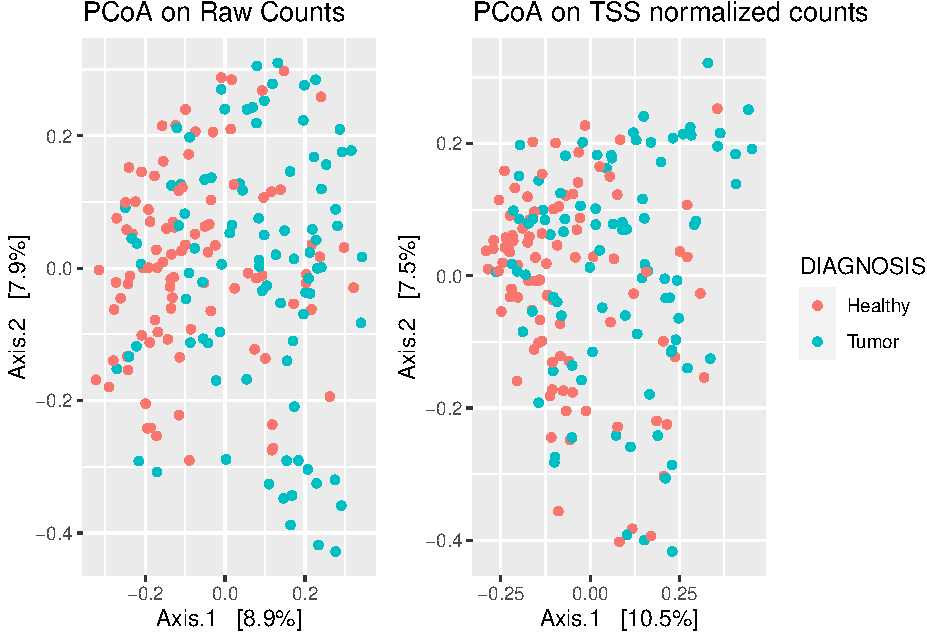
\includegraphics{MB_normalization_review_files/figure-latex/unnamed-chunk-10-1.pdf}

View how TMM normalization changes distance metrics differently than raw counts.

\begin{Shaded}
\begin{Highlighting}[]
\KeywordTok{plot\_norm\_changes}\NormalTok{(gp\_tmm, gp\_raw,}
                  \DataTypeTok{x\_lab =} \StringTok{"Raw"}\NormalTok{, }\DataTypeTok{y\_lab =} \StringTok{"TMM"}\NormalTok{,}
                  \DataTypeTok{title =} \StringTok{"Distance metric comparision between TMM normalization and Raw counts "}\NormalTok{)}
\end{Highlighting}
\end{Shaded}

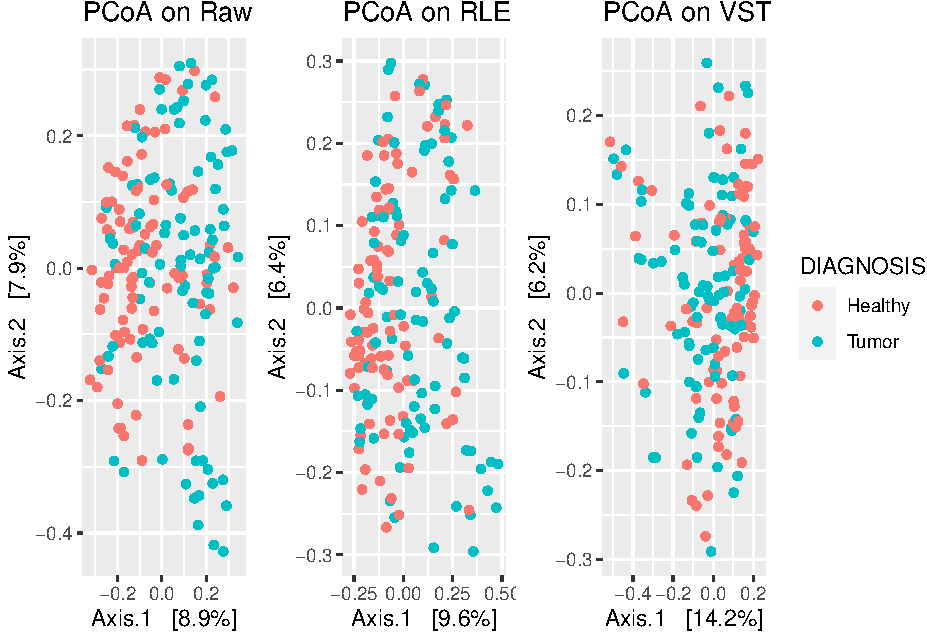
\includegraphics{MB_normalization_review_files/figure-latex/unnamed-chunk-11-1.pdf}

\hypertarget{cumulative-sum-scaling-css}{%
\chapter{Cumulative sum scaling (CSS)}\label{cumulative-sum-scaling-css}}

Cumulative sum scaling is a scaling normalization method, developed for marker gene sequencing, It is intended to account for undersampling and correct biases from preferentially amplified features in a sample-specific manner \citep{paulson2013}. This method assumes that count distributions should be roughly equivalent and independent to each other up to the given quantile which is chosen as the smallest value at which instability is found. This method is an extension to UQ scaling where a quantile is specified. If there is high count variability the assumption may not be met. This is not a method that accounts for compositionality. CSS normalization initially showed improvements in separating samples biologically in ordination, it was shown to be an artifact of unequal application of log transformation across methods \citep{costea2014}.

\hypertarget{css-implementation}{%
\section{CSS implementation}\label{css-implementation}}

\begin{Shaded}
\begin{Highlighting}[]
\NormalTok{norm\_CSS \textless{}{-}}\StringTok{ }\ControlFlowTok{function}\NormalTok{(ps)\{}
  \KeywordTok{require}\NormalTok{(metagenomeSeq)}
  \CommentTok{\# Convert to metagenomeSeq data type}
\NormalTok{  ps.metaG\textless{}{-}}\KeywordTok{phyloseq\_to\_metagenomeSeq}\NormalTok{(ps)}
\NormalTok{  p\_stat =}\StringTok{ }\KeywordTok{cumNormStatFast}\NormalTok{(ps.metaG)}
\NormalTok{  ps.metaG =}\StringTok{ }\KeywordTok{cumNorm}\NormalTok{(ps.metaG, }\DataTypeTok{p =}\NormalTok{ p\_stat)}
\NormalTok{  ps.metaG.norm \textless{}{-}}\StringTok{ }\KeywordTok{MRcounts}\NormalTok{(ps.metaG, }\DataTypeTok{norm =}\NormalTok{ T)}
  \CommentTok{\# Convert back to phyloseq with normalized counts}
\NormalTok{  otu \textless{}{-}}\StringTok{ }\KeywordTok{otu\_table}\NormalTok{(ps.metaG.norm, }\DataTypeTok{taxa\_are\_rows =}\NormalTok{ T)}
\NormalTok{  sam \textless{}{-}}\StringTok{ }\KeywordTok{access}\NormalTok{(ps, }\StringTok{"sam\_data"}\NormalTok{)}
\NormalTok{  sam}\OperatorTok{$}\NormalTok{scaling\_factor \textless{}{-}}\StringTok{ }\KeywordTok{normFactors}\NormalTok{(ps.metaG)}\OperatorTok{/}\FloatTok{1e6}
\NormalTok{  tax \textless{}{-}}\StringTok{ }\KeywordTok{access}\NormalTok{(ps, }\StringTok{"tax\_table"}\NormalTok{)}
\NormalTok{  phy \textless{}{-}}\StringTok{ }\KeywordTok{access}\NormalTok{(ps, }\StringTok{"phy\_tree"}\NormalTok{)}
\NormalTok{  ps\_CSS \textless{}{-}}\StringTok{ }\KeywordTok{phyloseq}\NormalTok{(otu,sam,tax,phy)}
  \KeywordTok{return}\NormalTok{(ps\_CSS)}
\NormalTok{\}}
\end{Highlighting}
\end{Shaded}

\hypertarget{css-on-global-patterns}{%
\section{CSS on Global Patterns}\label{css-on-global-patterns}}

Perform CSS normalization:

\begin{Shaded}
\begin{Highlighting}[]
\NormalTok{gp\_css \textless{}{-}}\StringTok{ }\KeywordTok{norm\_CSS}\NormalTok{(gp\_raw)}
\end{Highlighting}
\end{Shaded}

\begin{verbatim}
## Default value being used.
\end{verbatim}

View how TMM normalization changes distance metrics differently than raw counts.

\begin{Shaded}
\begin{Highlighting}[]
\KeywordTok{plot\_norm\_changes}\NormalTok{(gp\_css, gp\_raw, }
                  \DataTypeTok{x\_lab =} \StringTok{"Raw"}\NormalTok{, }\DataTypeTok{y\_lab =} \StringTok{"CSS"}\NormalTok{,}
                  \DataTypeTok{title =} \StringTok{"Distance metric comparision between CSS normalization and Raw counts"}\NormalTok{)}
\end{Highlighting}
\end{Shaded}

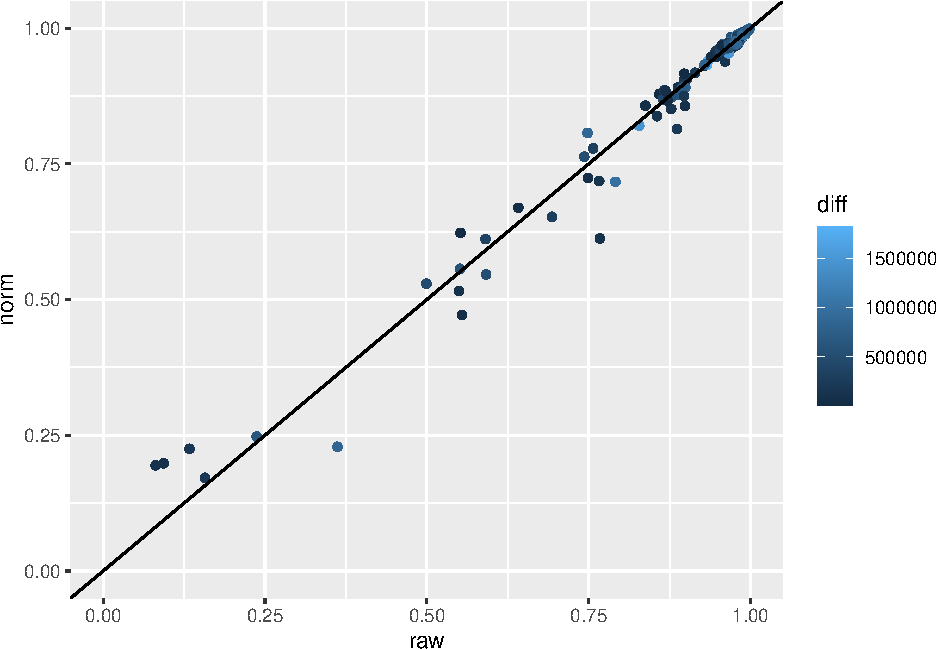
\includegraphics{MB_normalization_review_files/figure-latex/unnamed-chunk-14-1.pdf}

\begin{Shaded}
\begin{Highlighting}[]
\KeywordTok{plot\_norm\_changes}\NormalTok{(gp\_css, gp\_tss, }
                  \DataTypeTok{x\_lab =} \StringTok{"TSS"}\NormalTok{, }\DataTypeTok{y\_lab =} \StringTok{"CSS"}\NormalTok{,}
                  \DataTypeTok{title =} \StringTok{"Distance metric comparision between CSS normalization and TSS normalization"}\NormalTok{)}
\end{Highlighting}
\end{Shaded}

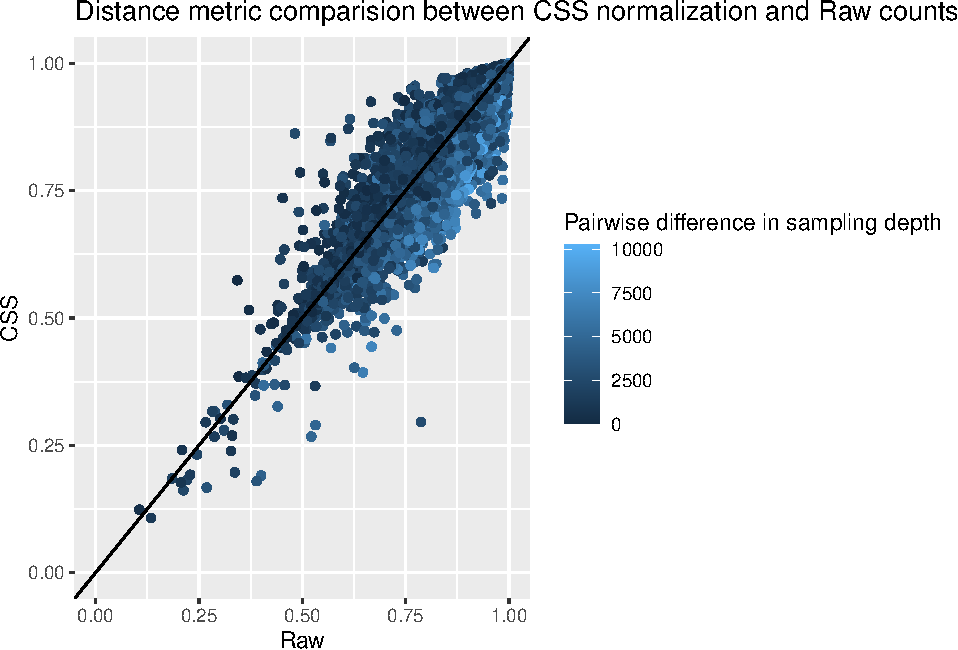
\includegraphics{MB_normalization_review_files/figure-latex/unnamed-chunk-14-2.pdf}

CSS normalization appears to consider pairs as more different than TSS normalization, and pairs with high sequencing depth differences even more so.

\hypertarget{gmpr}{%
\chapter{GMPR}\label{gmpr}}

A recent extension of the RLE DESeq method is the Geometric mean of Pairwise ratios (GMPR) approach \citep{chen2018}. This method reverses the steps of RLE, and instead calculates the median count ratio of the non-zero counts between pairs of samples as although only a small number of taxa are likely to be shared for every sample, it is more likely that there are many shared taxa between pairs. It then uses the pairwise results to calculate the size factor for each sample. This method has slow computation, but is robust to differential and outlier taxa. It addresses sparsity, but not composition. The size factors can be inputted to DESeq and a VST transformation applied additionally. It is a newer method, and has unfortunately not been included in many benchmarking studies, although initial results show it to be more powerful than DESeq, not surprisingly, as it uses more data, as zero counts do not need to be discarded. It assumes there is a large invariant portion of the count data, similar to other methods.

\hypertarget{gmpr-implementation}{%
\section{GMPR Implementation}\label{gmpr-implementation}}

\begin{Shaded}
\begin{Highlighting}[]
\NormalTok{norm\_GMPR \textless{}{-}}\StringTok{ }\ControlFlowTok{function}\NormalTok{(ps, }\DataTypeTok{scale =} \FloatTok{1e6}\NormalTok{)\{}
  \KeywordTok{require}\NormalTok{(GMPR, }\DataTypeTok{quietly =}\NormalTok{ T)}
    \CommentTok{\# Calculate GMPR size factor}
    \CommentTok{\# Row {-} features, column {-} samples}
\NormalTok{    otu \textless{}{-}}\StringTok{ }\KeywordTok{as}\NormalTok{(}\KeywordTok{otu\_table}\NormalTok{(ps), }\StringTok{"matrix"}\NormalTok{)}
    \ControlFlowTok{if}\NormalTok{(}\KeywordTok{taxa\_are\_rows}\NormalTok{(ps))\{otu \textless{}{-}}\StringTok{ }\KeywordTok{t}\NormalTok{(otu)\}}
\NormalTok{    otu\_df =}\StringTok{ }\KeywordTok{as.data.frame}\NormalTok{(otu)}
\NormalTok{    otu.tab \textless{}{-}}\StringTok{ }\KeywordTok{matrix}\NormalTok{(otu, }\DataTypeTok{ncol =} \KeywordTok{ncol}\NormalTok{(otu))}
\NormalTok{    gmpr.size.factor \textless{}{-}}\StringTok{ }\NormalTok{GMPR}\OperatorTok{::}\KeywordTok{GMPR}\NormalTok{(otu\_df, }\DataTypeTok{intersect\_no =} \DecValTok{4}\NormalTok{, }\DataTypeTok{min\_ct =} \DecValTok{2}\NormalTok{)}
    
    \CommentTok{\# normalize}
\NormalTok{    otu.tab.norm \textless{}{-}}\StringTok{ }\KeywordTok{t}\NormalTok{(}\KeywordTok{t}\NormalTok{(otu) }\OperatorTok{/}\StringTok{ }\NormalTok{(gmpr.size.factor}\OperatorTok{/}\NormalTok{scale))}
    
    \CommentTok{\# convert back to PS}
\NormalTok{    sam \textless{}{-}}\StringTok{ }\KeywordTok{access}\NormalTok{(ps, }\StringTok{"sam\_data"}\NormalTok{)}
\NormalTok{    sam}\OperatorTok{$}\NormalTok{scaling\_factor \textless{}{-}}\StringTok{ }\NormalTok{gmpr.size.factor}
\NormalTok{    tax \textless{}{-}}\StringTok{ }\KeywordTok{access}\NormalTok{(ps, }\StringTok{"tax\_table"}\NormalTok{)}
\NormalTok{    phy \textless{}{-}}\StringTok{ }\KeywordTok{access}\NormalTok{(ps, }\StringTok{"phy\_tree"}\NormalTok{)}
\NormalTok{    ps\_GMPR \textless{}{-}}\StringTok{ }\KeywordTok{phyloseq}\NormalTok{(}\KeywordTok{otu\_table}\NormalTok{(otu.tab.norm, }\DataTypeTok{taxa\_are\_rows =}\NormalTok{ F),sam,tax,phy)}
    \KeywordTok{return}\NormalTok{(ps\_GMPR)}
\NormalTok{\}}
\end{Highlighting}
\end{Shaded}

\hypertarget{global-patterns-gmpr}{%
\section{Global Patterns GMPR}\label{global-patterns-gmpr}}

\begin{Shaded}
\begin{Highlighting}[]
\CommentTok{\# Normalize}
\NormalTok{gp\_gmpr \textless{}{-}}\StringTok{ }\KeywordTok{norm\_GMPR}\NormalTok{(gp\_raw)}


\CommentTok{\# Compare to other methods like before}
\KeywordTok{plot\_norm\_changes}\NormalTok{(gp\_gmpr, gp\_raw, }
                  \DataTypeTok{x\_lab =} \StringTok{"GMPR"}\NormalTok{, }\DataTypeTok{y\_lab =} \StringTok{"Raw Counts"}\NormalTok{,}
                  \DataTypeTok{title =} \StringTok{"GMPR normalization vs Raw Counts"}\NormalTok{)}
\end{Highlighting}
\end{Shaded}

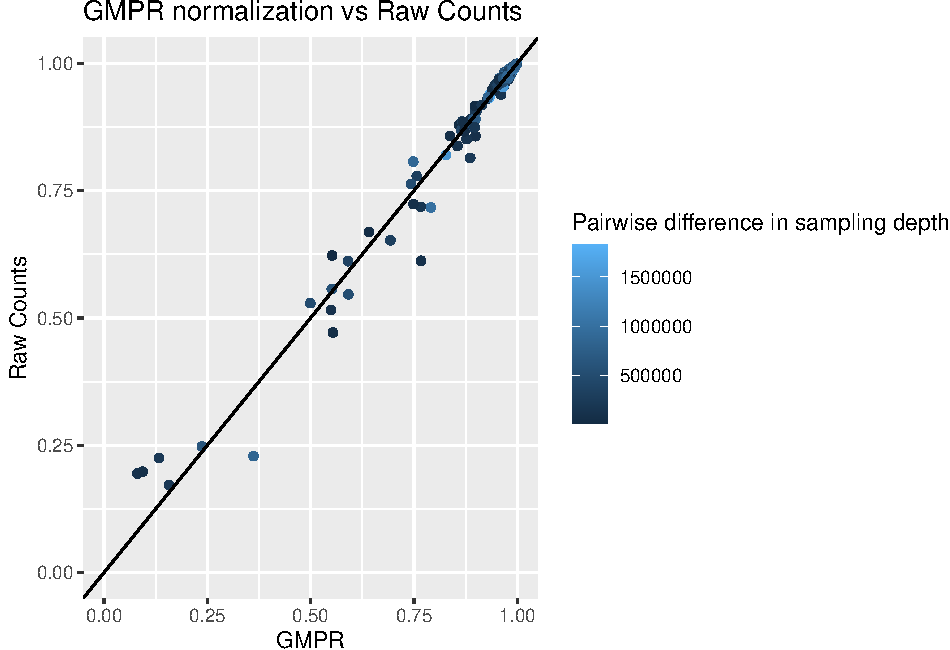
\includegraphics{MB_normalization_review_files/figure-latex/unnamed-chunk-16-1.pdf}

\begin{Shaded}
\begin{Highlighting}[]
\KeywordTok{plot\_norm\_changes}\NormalTok{(gp\_gmpr, gp\_tss,}
                  \DataTypeTok{x\_lab =} \StringTok{"TSS"}\NormalTok{, }\DataTypeTok{y\_lab =} \StringTok{"GMPR"}\NormalTok{, }
                  \DataTypeTok{title =} \StringTok{"TSS vs GMPR"}\NormalTok{)}
\end{Highlighting}
\end{Shaded}

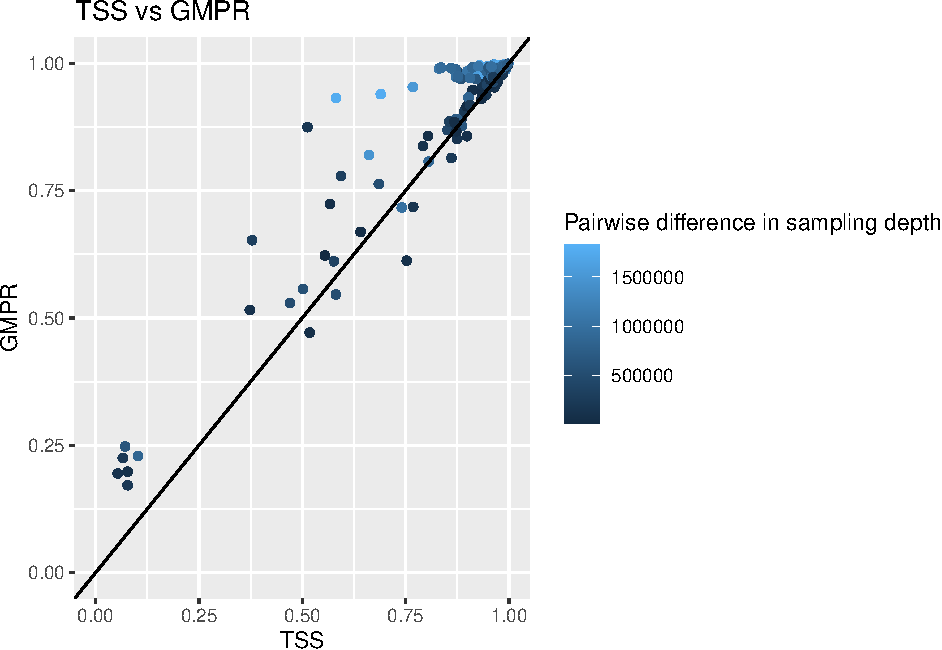
\includegraphics{MB_normalization_review_files/figure-latex/unnamed-chunk-16-2.pdf}

\begin{Shaded}
\begin{Highlighting}[]
\KeywordTok{plot\_norm\_changes}\NormalTok{(gp\_gmpr, gp\_css,}
                  \DataTypeTok{x\_lab =} \StringTok{"CSS"}\NormalTok{, }\DataTypeTok{y\_lab =} \StringTok{"GMPR"}\NormalTok{, }
                  \DataTypeTok{title =} \StringTok{"CSS vs GMPR"}\NormalTok{ )}
\end{Highlighting}
\end{Shaded}

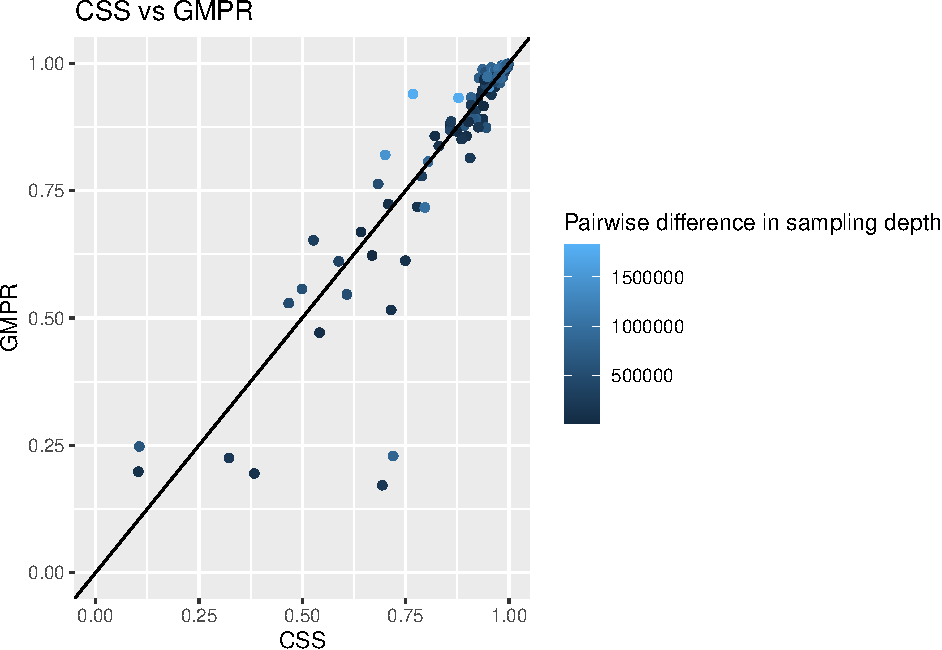
\includegraphics{MB_normalization_review_files/figure-latex/unnamed-chunk-16-3.pdf}

\hypertarget{wrench}{%
\chapter{Wrench}\label{wrench}}

Wrench is a recent normalization method developed for microbiome data \citep{kumar2018}. This method includes compositional bias correction for sparse datasets. This method uses a hurdle log-normal distribution to estimate the normalization factors (the location estimate for the group). For this method, we assume abundances are drawn from a hurdle Log-Gaussian distribution, and the scaling factor used is essentially the location estimate for the group.

\hypertarget{wrench-implementation}{%
\section{Wrench Implementation}\label{wrench-implementation}}

\begin{Shaded}
\begin{Highlighting}[]
\NormalTok{norm\_wrench \textless{}{-}}\StringTok{ }\ControlFlowTok{function}\NormalTok{(ps, group\_col)\{}
    \KeywordTok{require}\NormalTok{(Wrench, }\DataTypeTok{quietly =}\NormalTok{ T)}
    \ControlFlowTok{if}\NormalTok{( }\KeywordTok{identical}\NormalTok{(}\KeywordTok{all.equal}\NormalTok{(}\KeywordTok{length}\NormalTok{(group\_col), }\DecValTok{1}\NormalTok{), }\OtherTok{TRUE}\NormalTok{) }\OperatorTok{\&}\StringTok{ }\KeywordTok{nsamples}\NormalTok{(ps) }\OperatorTok{\textgreater{}}\StringTok{ }\DecValTok{1}\NormalTok{ )\{}
        \CommentTok{\# Assume that group was a sample variable name (must be categorical)}
\NormalTok{        group =}\StringTok{ }\KeywordTok{get\_variable}\NormalTok{(ps, group\_col)}
\NormalTok{    \}}
\NormalTok{    otu\_tab \textless{}{-}}\StringTok{ }\KeywordTok{otu\_table}\NormalTok{(ps)}
\NormalTok{    W \textless{}{-}}\StringTok{ }\KeywordTok{wrench}\NormalTok{(otu\_tab, group)}
    
\NormalTok{    compositionalFactors \textless{}{-}}\StringTok{ }\NormalTok{W}\OperatorTok{$}\NormalTok{ccf}
\NormalTok{    normalizationFactors \textless{}{-}}\StringTok{ }\NormalTok{W}\OperatorTok{$}\NormalTok{nf}
    
\NormalTok{    normed\_otu \textless{}{-}}\StringTok{ }\NormalTok{otu\_tab}\OperatorTok{/}\NormalTok{(normalizationFactors}\OperatorTok{/}\FloatTok{1e6}\NormalTok{)}
\NormalTok{    otu \textless{}{-}}\StringTok{ }\KeywordTok{otu\_table}\NormalTok{(normed\_otu, }\DataTypeTok{taxa\_are\_rows =}\NormalTok{ T)}
\NormalTok{    sam \textless{}{-}}\StringTok{ }\KeywordTok{access}\NormalTok{(ps, }\StringTok{"sam\_data"}\NormalTok{)}
\NormalTok{    sam}\OperatorTok{$}\NormalTok{scaling\_factor \textless{}{-}}\StringTok{ }\NormalTok{normalizationFactors}
\NormalTok{    tax \textless{}{-}}\StringTok{ }\KeywordTok{access}\NormalTok{(ps, }\StringTok{"tax\_table"}\NormalTok{)}
\NormalTok{    phy \textless{}{-}}\StringTok{ }\KeywordTok{access}\NormalTok{(ps, }\StringTok{"phy\_tree"}\NormalTok{)}
\NormalTok{    ps\_wrench \textless{}{-}}\StringTok{ }\KeywordTok{phyloseq}\NormalTok{(otu,sam,tax,phy)}
    
    \KeywordTok{return}\NormalTok{(ps\_wrench)}
\NormalTok{\}}
\end{Highlighting}
\end{Shaded}

\hypertarget{wrench-on-global-patterns}{%
\section{Wrench on Global Patterns}\label{wrench-on-global-patterns}}

\begin{Shaded}
\begin{Highlighting}[]
\NormalTok{gp\_wrench \textless{}{-}}\StringTok{ }\KeywordTok{norm\_wrench}\NormalTok{(gp\_raw, }\DataTypeTok{group\_col =} \StringTok{"SampleType"}\NormalTok{)}
\end{Highlighting}
\end{Shaded}

\hypertarget{comparisions}{%
\chapter{Comparisions}\label{comparisions}}

\begin{Shaded}
\begin{Highlighting}[]
\KeywordTok{library}\NormalTok{(GGally)}
\end{Highlighting}
\end{Shaded}

\begin{verbatim}
## Registered S3 method overwritten by 'GGally':
##   method from   
##   +.gg   ggplot2
\end{verbatim}

\begin{Shaded}
\begin{Highlighting}[]
\KeywordTok{data.frame}\NormalTok{(}\DataTypeTok{raw =} \KeywordTok{as.numeric}\NormalTok{(phyloseq}\OperatorTok{::}\KeywordTok{distance}\NormalTok{(gp\_raw, }\StringTok{"bray"}\NormalTok{)), }
           \DataTypeTok{tss =} \KeywordTok{as.numeric}\NormalTok{(phyloseq}\OperatorTok{::}\KeywordTok{distance}\NormalTok{(gp\_tss, }\StringTok{"bray"}\NormalTok{)), }
           \DataTypeTok{css =} \KeywordTok{as.numeric}\NormalTok{(phyloseq}\OperatorTok{::}\KeywordTok{distance}\NormalTok{(gp\_css, }\StringTok{"bray"}\NormalTok{)),}
           \DataTypeTok{deseq\_rle =} \KeywordTok{as.numeric}\NormalTok{(phyloseq}\OperatorTok{::}\KeywordTok{distance}\NormalTok{(gp\_deseq\_rle, }\StringTok{"bray"}\NormalTok{)),}
           \DataTypeTok{deseq\_vs =} \KeywordTok{as.numeric}\NormalTok{(phyloseq}\OperatorTok{::}\KeywordTok{distance}\NormalTok{(gp\_deseq\_vs, }\StringTok{"bray"}\NormalTok{)),}
           \DataTypeTok{rare =} \KeywordTok{as.numeric}\NormalTok{(phyloseq}\OperatorTok{::}\KeywordTok{distance}\NormalTok{(gp\_rare, }\StringTok{"bray"}\NormalTok{)),}
           \DataTypeTok{tmm =} \KeywordTok{as.numeric}\NormalTok{(phyloseq}\OperatorTok{::}\KeywordTok{distance}\NormalTok{(gp\_tmm, }\StringTok{"bray"}\NormalTok{)),}
           \DataTypeTok{diff =} \KeywordTok{as.numeric}\NormalTok{(}\KeywordTok{dist}\NormalTok{(}\KeywordTok{get\_variable}\NormalTok{(gp\_raw, }\StringTok{"depth"}\NormalTok{)))) }\OperatorTok{\%\textgreater{}\%}\StringTok{ }
\StringTok{    }\KeywordTok{ggpairs}\NormalTok{(}\DataTypeTok{columns =} \DecValTok{1}\OperatorTok{:}\DecValTok{7}\NormalTok{, }\DataTypeTok{upper =} \StringTok{"blank"}\NormalTok{,}
            \DataTypeTok{diag =} \StringTok{"blank"}\NormalTok{,ggplot2}\OperatorTok{::}\KeywordTok{aes}\NormalTok{(}\DataTypeTok{colour=}\NormalTok{diff))}
\end{Highlighting}
\end{Shaded}

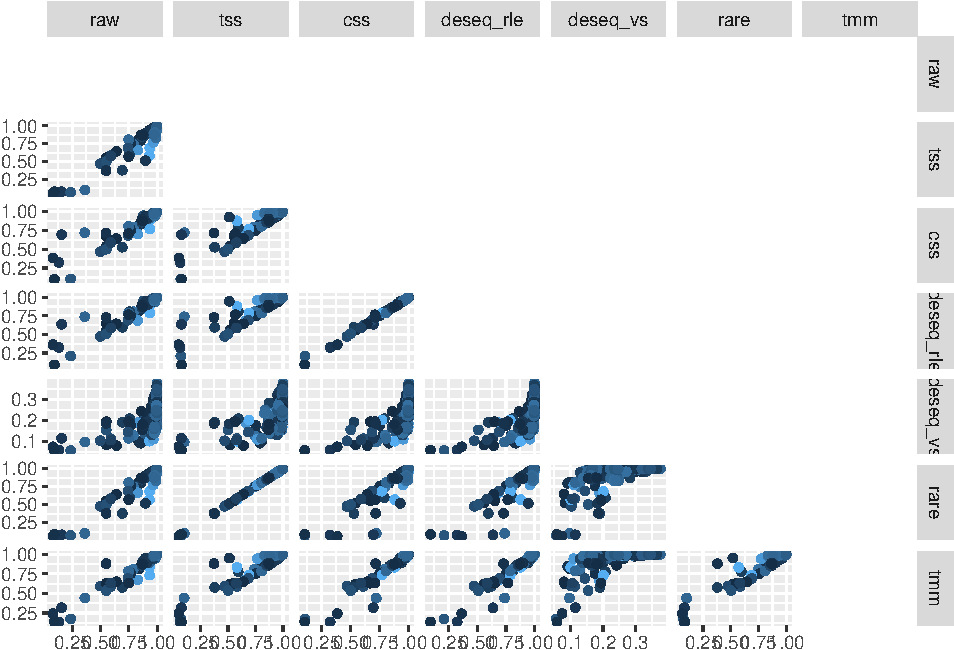
\includegraphics{MB_normalization_review_files/figure-latex/unnamed-chunk-20-1.pdf}

  \bibliography{book.bib,packages.bib}

\end{document}
